\section{Обсуждение}
\label{sec:discussion}

\subsection{Обзор ключевых результатов}

Данные $N = 1426$ поддерживают шестифакторную архитектуру с тремя уровнями различений, не сводимых друг к другу. Первый уровень --- содержательные конструкты психики: внутренний диссонанс (ID) как признак блокирующей защитной работы, детское отчуждение (CA) как средовой анамнез, психопатия (P) как моральная подпись «мне разрешено», аффективная и когнитивная эмпатия (\EAF{}, \Ecog{}) как две различимые функции, маскирование (M) как регуляторный слой. Второй уровень --- их структурная геометрия: ID и P статистически разделимы и описывают два разных канала потери эмпатии (пассивная блокировка и активный нарратив), \Ecog{} и \EAF{} не эквивалентны и диссоциируются под разными условиями, M --- слабый, плохо дифференцированный фактор ($\omega = 0.546$), заведомо не готовый к самостоятельным выводам. Третий уровень --- внимание (A) как структурно иной элемент: не содержание психики, а условие её организации. Именно A модерирует оба участка канала CA$\to$ID$\to$\EAF{} в узкой спецификации и преобразует классическую картину травматического повреждения в профиль интегрированного выжившего. Эти результаты воспроизводят то, что было описано в разных литературах по отдельности, но не были объединены в одной психометрической ткани.

\paragraph{Центральный эмпирический сдвиг: ломает эмпатию не травма, а защита.} Прежде чем переходить к прочтению факторов, мы выносим наверх один результат, который переформулирует вековую клиническую интуицию. В базовой регрессионной модели CA напрямую отрицательно предсказывает \EAF{} (total effect $c = -0.129$, 95\% CI $[-0.184, -0.073]$) --- знак, согласованный со стандартной картиной «травма подавляет эмпатию». Но как только мы включаем ID как медиатор, прямой эффект CA на \EAF{} \emph{меняет знак} на положительный ($c' = +0.073$, 95\% CI $[+0.018, +0.128]$). Иначе говоря: если защитная структура, которую травма построила, не учитывается, связь между детской историей и сниженной взрослой эмпатией видна; если защитную структуру учесть --- детская история сама по себе связана с аффективной эмпатией слабо положительно, а негативный эффект полностью проходит через канал ID. Это не статистический артефакт и не косметика --- это смещение каузальной точки приложения терапии: работать надо не с прошлым как таковым, а с защитой, выстроенной между прошлым и настоящим. Клиническая интуиция, существовавшая со времён \citet{freud1917}, что «травма требует повторной переработки» (Durcharbeiten), получает операциональное уточнение --- перерабатывать нужно не событие, а защитную структуру, оставленную событием. Это же основание для тезиса §\ref{subsec:integrated_survivor} об интегрированном выжившем: когда защитная структура метаболизирована, \emph{положительная} компонента связи CA $\to$ \EAF{} становится наблюдаемой на уровне группы, а не только скрытым статистическим остатком.

\paragraph{Откуда возникла эта архитектура.} Текущая латентная формулировка не была началом программы. Пилотная композитная версия инструмента (DEIC-DRAFT, август 2025, 14 содержательных осей, с самостоятельными подшкалами S / D / AIS / F / IDS внутри защитного контура) в парциально-корреляционных анализах, корректированных на Lie-шкалу и ковариаты, дала два устойчивых парадокса. Первый --- неожиданно слабая связь эмпатии с внутренним диссонансом: если E и IDS --- два независимых конструкта, прямая модель «диссонанс блокирует чувствование» предсказывает систематически отрицательную корреляцию, которой в данных не оказывалось. Второй --- спорадически положительные частные корреляции E с отдельными индикаторами пассивного блокирования: если D блокирует E, знак должен быть устойчиво отрицательным, а не знакопеременным. В композитной рамке оба наблюдения читались как ошибка. В текущей латентной условной рамке оба --- предсказуемые следствия: композиты склеивали то, что архитектурно разделимо. Эмпатия как state (аффективный резонанс, \EAF{}) реагирует на защитную структуру не так, как эмпатия как декларация (\Ecog{} или trait-установка); ID-блок включается не автоматически, а условно через witnessing. Оба парадокса оказываются частными случаями одной геометрии, и именно это --- а не добавление новых данных --- сделало переход от композитной модели к латентной условной архитектуре обязательным, а не косметическим.

Мы не предлагаем новую теорию эмпатии. Мы предлагаем \emph{каркас измерения}, в котором уже описанные в разных традициях конструкты получают общие координаты и проверяемые взаимные отношения. Это не значит, что модель метафизически нейтральна --- любое измерение содержит онтологическое обязательство относительно того, что оно измеряет. Мы это обязательство не прячем за риторикой «мы всего лишь психометрики». Мы утверждаем прямо: шесть функций \DEIC{} соответствуют реальной структуре в слабом, но конкретном смысле --- эта структура порождает предсказания, которые могут не сбыться, и если не сбываются в предрегистрированной репликации, модель в соответствующей точке опровергнута. То, что мы не заявляем, --- это готовую теорию психики в целом; то, что мы заявляем, --- что измеренное коррелирует с тем, что есть.

\subsection{Три точки эмпирического сопротивления рамке}
\label{subsec:data_resistance}

Worldview-first работа (см. §\ref{subsec:worldview_first}) имеет право на существование в той мере, в которой данные сопротивляются исходной рамке в конкретных, центральных местах. Мы выделяем эти места явно, потому что в параграфах результатов они разбросаны и их суммарный вес легко потерять.

\paragraph{Первое --- коллапс \IMM{} в unified-SEM.} В узкой спецификации канала CA$\to$ID$\to$\EAF{} с A как двойным модератором обеих стадий $\IMM = -0.00197$ со значимым бутстрэповским CI. Это было одно из центральных ожидаемых подтверждений: A должно перестраивать канал целиком. В unified-SEM, где P, A, M включены одновременно как параллельные медиаторы и main-effects, \IMM{} коллапсирует до $+0.0001$ (NS). Это не артефакт и не шум --- это ре-композиция дисперсии: основной объяснительной силой \EAF{} на популяционном уровне обладает не произведение ID$\times$A, а P как прямой негативный предиктор ($b = -0.726$) и A как прямой позитивный предиктор ($b = +0.393$). Мы были вынуждены переформулировать: ID-A-модуляция остаётся содержательно значимой на уровне индивидуальной траектории (§\ref{subsec:architecture}), но population-level основная дисперсия аффективной эмпатии концентрируется в P-нарративе и A-присутствии. Это более слабое утверждение, чем мы начинали формулировать.

\paragraph{Второе --- SUP отказывается быть частью пассивного блокирования.} Пять wave-1 защитных шкал в исходной рамке должны были собираться в единый латент ID как разные поверхности одной контейнирующей системы. Бифакторный анализ показал: per-subscale ECV для SUP $= 0.31$ (69\% дисперсии подавления уникальна и не объясняется общим ID), композитные корреляции SUP $\leftrightarrow$ IDS $= 0.05$ и SUP $\leftrightarrow$ DIS $= 0.11$. При этом на тех же parcel-композитах $r(\mathrm{SUP}, P) = +0.245$ и $r(\mathrm{SUP}, M) = +0.348$: подавление коррелирует с P и M \emph{сильнее}, чем с любой из четырёх шкал пассивного блокирования, в пакет которых оно было заведено по дизайну. Феноменологически это встаёт на место: подавление --- эго-синтонное сознательное действие, в котором субъект \emph{выбирает} не чувствовать, и структурно оно ближе к P-архитектуре условного доступа и к M-регуляции фасада, чем к диссоциации, изоляции, уплощённости как автоматическим эго-дистонным механизмам. В рамке до данных SUP и DIS трактовались как изоморфные индикаторы одной системы; после данных SUP должен быть вынесен в отдельный латент в волне 2, и его естественное место --- рядом с P и M в кластере сознательно-волевой регуляции аффекта, а не внутри ID. Это не уточнение внутри рамки, это изменение самой топологии защит.

\paragraph{Третье --- A отказывается быть латентом.} Мы ожидали, что witnessing ведёт себя как обычный рефлексивный латент: набор пунктов, загружающихся на общий фактор внимания. A-CFA Tier~5 с очищенным набором из 17 пунктов даёт CFI $= 0.87$, RMSEA $= 0.08$ --- и, концептуально важнее, сигнатурное \emph{перевёртывание знака} \IMM{} при использовании латентного A вместо композитного. Перевёртывание знака при очистке конструкта --- диагностический признак формативной, а не рефлексивной структуры: у A нет общего дисперсионного ядра, которое можно было бы извлечь из пунктов, потому что A --- не внутренняя черта, которая проявляется в поведении, а поле-условие, в котором существуют другие функции (§\ref{subsec:A_as_field_condition}). Это наиболее значимое из трёх изменений: оно переводит центральный модератор программы из обычного психометрического конструкта в онтологически другой тип объекта. Волна 2 требует отдельной A-шкалы, сконструированной формативно по дизайну, с явной работой с методологическими последствиями этого выбора.

Эти три точки --- не дежурный перечень ограничений. Это места, в которых данные заставили рамку реально изогнуться: ожидаемый эффект исчез, ожидаемая структура распалась, ожидаемый тип конструкта оказался иным. Именно наличие этих трёх сдвигов --- основное имеющееся у нас свидетельство того, что рамка не самоподтверждается. Если бы данные не сопротивлялись нигде, работу стоило бы читать как декоративную эмпирику. Они сопротивлялись, и сопротивление названо.

\subsection{Что дают три новых валидационных среза вместе}
\label{subsec:validity_package}

Три подсекции §\ref{subsec:free_text_convergent}, \ref{subsec:roc_validity} и \ref{subsec:dx_count_bias} адресуют один и тот же вопрос с трёх независимых сторон: насколько конструкты DEIC измеряют то, что они называются, и что именно они измеряют по сравнению со стандартными клиническими проксами. Эти три результата мы выносим в обсуждение как единый пакет, потому что по отдельности они читаются как технические валидационные отчёты, а вместе --- как структурное утверждение.

\emph{Конвергентно} P-шкала подтверждается прямым текстовым самоописанием (manipulation\_callousness $N = 10$, $d_P = +2.32$, AUC $= 0.964$), причём P удерживает значимость в многофакторной модели с полным набором ковариат. \emph{Архитектурно} разделение каналов P и ID воспроизводится на поведенческих якорях: manipulation\_callousness активирует P без D, social\_isolation --- D без P. Эти два полюса --- эмпирические «crystalline examples» двух контуров, о которых модель говорит. \emph{Дискриминантно} P демонстрирует систематически сниженную ROC ($\mathrm{AUC} \leq 0.42$) для всех восьми self-report диагностических категорий: конструкт, измеряющий архитектуру условного доступа и моральный нарратив «мне разрешено», по определению не должен предсказывать обращение за диагнозом; он предсказывает его \emph{отсутствие}, и это эмпирически подтверждается. Симметрично CA демонстрирует $\mathrm{AUC} = 0.69$--$0.76$ для трёх раннетравматических кластеров (trauma, self-harm, personality); A даёт $\mathrm{AUC} \leq 0.46$ для большинства кластеров как ресурс-предиктор отсутствия клинической декомпенсации.

Три подписи когерентны. Они означают: \DEIC{} не замещает DSM и не сводим к нему. DEIC измеряет ось, структурно \emph{ортогональную} логике self-report клинического диагноза: P-респонденты архитектурно невидимы для dx-центрированных инструментов, CA-респонденты --- архитектурно видимы через раннетравматическую подпись, A-респонденты --- архитектурно защищены от декомпенсации. Это --- эмпирическое обоснование того, почему в клинике имеет смысл использовать DEIC \emph{рядом} с стандартной диагностикой, а не вместо неё или как её upstream-прокси. DEIC ловит то, что self-report DSM не ловит; self-report DSM ловит то, что DEIC специфично \emph{не} ловит.

Вторая импликация --- методологическая. $\texttt{dx\_count}$ как мера тяжести в DEIC-популяции смещён архитектурно, не только статистически: он монотонно растёт с раннетравматической осью, но падает с активным P-профилем, то есть встраивает в себя ту самую асимметрию видимости, которую конструкт P описывает. В статье мы используем $\texttt{dx\_count}$ только для описательной характеристики выборки; формальная клиническая валидизация требует wave с структурированной диагностикой (§\ref{subsec:wave2_design}).

\subsection{Архитектура шести факторов --- короткое прочтение}

\textbf{ID (внутренний диссонанс)} --- не «симптом», а признак того, что регуляция активна и работает в режиме блокировки. Высокий ID означает, что внутри психики присутствует конфликт, и часть аффективного контента сигнализирует о своём подавлении. В терминах психоанализа это то, что \citet{ferenczi1933} и \citet{klein1946} описывали как расщепление и отщепление; в терминах теории привязанности --- дезорганизованные внутренние рабочие модели \citep{main1986}. Наш вклад --- психометрическая координата, которую можно измерить, воспроизвести и соотносить с исходами.

\textbf{CA (детское отчуждение)} --- узкий средовой предшественник, не полный синдром ACE. Это именно \emph{переживание несоответствия} в семье первых лет: когда внутренние состояния ребёнка не встречают адекватного отклика, и поле семьи становится структурно несовместимым с собственным эмоциональным опытом. В наших данных CA сильнее предсказывает ID и дистанцирование, чем общий ACE-индекс. Это согласуется с теорией mentalization \citep{fonagy2002}: не травма сама по себе, а отсутствие ментализующего отклика формирует предрасположенность.

\textbf{P (психопатия)} --- моральный нарратив «это разрешено мне». В \DEIC{} этот конструкт \emph{отдельно} от архитектуры аффективного сцепления (см. §\ref{subsec:architecture}): P --- слой разрешения, не слой способности. Partial $r$(P, \Ecog{}) после partialling ID и CA = $+0.32$ --- то есть у людей с высоким P когнитивная эмпатия скорее \emph{повышена}, чем понижена. Это совместимо с тем, что описали \citet{blair1995, blair2013} и \citet{baroncohen2011}: психопатический паттерн включает нарративный слой самооправдания как самостоятельный конструкт, не производный от аффективного уровня. В нашей формулировке --- «способность понимать других, не чувствуя моральной обязанности» --- это не описание разрушенной функции, а описание конкретной комбинации архитектуры (условное сцепление) и нарратива (разрешение). Работа \citet{cleckley1941} --- первое литературное описание этой структуры. Этот паттерн --- когнитивная эмпатия сохранна или повышена при заблокированном аффективном резонансе --- в пилотной композитной формулировке инструмента фиксировался как \emph{«тёмная зона эмпатии»}. В латентной рамке имя уточняется: не «тёмная зона» внутри эмпатии, а \emph{топологическая зона}, в которой два разделимых канала (\Ecog{} и \EAF{}) сцеплены не друг с другом, а с разными уровнями архитектуры; P-нарратив определяет, во что эта разведённость разворачивается на поведенческом выходе --- от хищничества до точной клинической работы с высоким аффективным содержанием без со-паралича.

\textbf{\EAF{} / \Ecog{}} --- в оригинальном инструменте частично смешаны; post-hoc факторное разделение разрешило парадокс $r_{\mathrm{latent}}(P, E) = +0.35$ в оригинальной модели. Шкалы волны 2 должны эти два конструкта развести по дизайну. \citet{shamaytsoory2011} в нейропсихологической литературе эту диссоциацию защищает; наша психометрия её независимо воспроизводит.

\textbf{M (маскирование)} --- регуляторный слой между внутренним состоянием и его внешним предъявлением. В текущем инструменте M инструментирован слабо и неточно дифференцирован от P ($r_{\mathrm{latent}} = +0.82$); надёжность $\omega = 0.546$ не позволяет делать M-специфические выводы. Мы сохраняем M в модели как место под будущую шкалу, но не делаем на него ставку в данной статье.

\textbf{A (внимание)} --- устанавливается отдельно в следующем разделе, потому что имеет особый онтологический статус.

Ключевая геометрия между этими факторами такова: P и ID ортогональны (разные механизмы потери эмпатии), \EAF{} и \Ecog{} разделимы (разные функции эмпатии), CA предшествует ID во временной причинности (возраст-стратифицированные медиации устойчивы), и A модерирует обе стадии канала CA$\to$ID$\to$\EAF{} в узкой спецификации.

\subsection{A как условие поля, не содержание поля}
\label{subsec:A_as_field_condition}

Самое глубокое теоретическое различение в архитектуре \DEIC{} заключается не в том, \emph{какие} факторы входят в модель, а в том, что \emph{не все они имеют одинаковый онтологический статус}. ID, CA, P, M, \EAF{}, \Ecog{} --- содержательные факторы, отвечающие на вопрос «что присутствует в психике этого человека». Внимание (A) --- структурно иной фактор, отвечающий на другой вопрос: «есть ли внутри этой психики наблюдающее отношение как таковое». Это различие не лексическое.

Эмпирический след этого различия --- три независимых результата. Во-первых, попытка выстроить higher-order «Integration» фактор над \{A, $-$M, \EAF{}, $-$ID\} даёт катастрофически плохой fit (CFI = 0.71, RMSEA = 0.55), а корреляция полученного INT\_score с A равна 0.995. Это значит, что «интеграции» как отдельного конструкта над A не существует --- A и есть интеграция, измеренная нашей композитной процедурой. Во-вторых, conditional process SEM с A-композитом в качестве модератора показывает, что A не просто добавляется как предиктор, но \emph{перестраивает} канал CA$\to$ID$\to$\EAF{}. Индекс моделируемой модерации $\IMM = -0.00197$, 95\% CI $[-0.00533, -0.00005]$ --- значим в узкой спецификации, и при высоких значениях A канонический путь ущерба меняет знак. В-третьих, самый сильный аргумент --- A-CFA Tier 5 на тщательно отобранных 17 метакогнитивных айтемах даёт приемлемый fit (CFI = 0.866, RMSEA = 0.081) и высокую надёжность ($\omega$ по абсолютным нагрузкам = 0.947), но обнаруживает \emph{биполярную} факторную структуру: 8 айтемов грузят в одну сторону, 9 --- в противоположную, несмотря на априорное выравнивание полярности. Когда этот латентный A подставляется в тот же conditional process SEM вместо теоретически взвешенного композита, знаки главных коэффициентов переворачиваются (A $\to$ ID переходит от $-0.626$ к $+0.659$), и \IMM{} теряет значимость.

Мы предпочли не прятать этот результат, а сделать его центром раздела. Он означает следующее: в текущем пуле айтемов метакогнитивной формулировки «я замечаю свои внутренние состояния» совмещены два разных конструкта. Один --- собственно \emph{witnessing}, наблюдение-наблюдения, свидетельствующее отношение, которое функционально ослабляет сцепку ID$\leftrightarrow$\EAF{}-подавление. Другой --- \emph{trauma hypervigilance}, болезненная гипербдительность к внутренним состояниям, которая коррелирует с ID положительно и характеризует именно травмированное, а не интегрированное состояние. Голая CFA их не различает; теоретически взвешенный композит, в который это различие вложено заранее, --- различает.

Из этого следует методологический вывод, который мы делаем \emph{эмпирическим основанием} нашей позиции, а не оговоркой: A в текущем инструменте --- формативный, а не рефлексивный конструкт. Главный результат (\IMM{} сквозь A-модерацию) получен при теоретически корректном взвешивании; робастность-проверка на голом латентном A показывает, что witnessing как отдельный конструкт нужно инструментировать заново, с айтемами, специально различающими наблюдение-наблюдения от внутренней гипервнимательности. Это и есть приоритет первой очереди для волны 2.

\paragraph{Эмпатическое внимание: содержательное имя для прикладного регистра.} Ретроспективно: в парциально-корреляционных анализах композитной пилотной версии A проявлялось не как самостоятельная черта, а как модификатор всех остальных связей эмпатии с защитами --- при partialling A паттерны E$\leftrightarrow$\{S, D, AIS, F\} перестраивались нелинейно. Этот рабочий феномен получал тогда название \emph{эмпатического внимания}: внимания, меняющего геометрию аффективных связей, а не добавляющегося к ним как ещё одна черта. Текущая формулировка «A как field-condition, not field-content» --- онтологически отчётливое прочтение того же эмпирического следа: A не увеличивает E, A устанавливает поле, в котором \EAF{} может или не может быть сцеплено с ID-блокировкой. Имя \emph{эмпатическое внимание} остаётся содержательно точным для прикладного клинического регистра, где термин «field-condition» звучит абстрактно, --- и оно встаёт в один ряд с операциональным значением \textit{sākṣī}, \textit{rigpa} и «самовоспоминания» (§далее в этом разделе), а не с поведенческим mindfulness-skill.

Что witnessing --- структурно иной слой, а не ещё один контент психики, --- утверждение, которое различные линии мысли делали независимо и на протяжении по меньшей мере двух с половиной тысяч лет. Мы не обходим эту литературу и не делаем из неё декоративный фон; мы работаем в её корпусе напрямую. В адвайта-веданте это \textit{sākṣī}, свидетель, --- тот слой, в котором наблюдаются все остальные состояния и который сам не есть состояние \citep[через][]{godman1985, nisargadatta1973}. В дзогчене это \textit{rigpa}, изначальное осознавание, отличаемое от \textit{sems} (обычного ума-содержания) как структурно иной режим сознания. В буддийской \textit{satipaṭṭhāna}-традиции это mindfulness в её исходном, не редуцированном до behavioral-skill виде: припоминание присутствия, а не техника концентрации. У Гурджиева --- «самовоспоминание» \citep[через][]{ouspensky1949}, прямое требование удерживать наблюдающее отношение одновременно с наблюдаемым действием; в текстах Четвёртого пути эта функция отделяется от эмоциональных и когнитивных функций как структурно автономная. В психоанализе та же асимметрия проступает в «наблюдающем Я» \citep{sterba1934, kris1956} и получает современную форму в ментализации у \citet{fonagy2002}. В когнитивной науке последних двух десятилетий --- мета-осознанность как отдельная способность, описанная \citet{dunne2011} на буддийско-философской основе, \citet{josipovic2014} в non-dual рамке, \citet{grabovac2011} в их Buddhist Psychological Model. \citet{lutz2008} прямо показывают, что современная клиническая mindfulness-наука унаследовала только одну из нескольких различимых функций оригинальной конструкции.

Мы называем эти линии не как «аллюзии» и не как «параллельные описания», которые \DEIC{} якобы собирает в единую карту. Мы называем их потому, что каждая из них в своей системе работает с тем же структурным различением, которое в наших данных проступает эмпирически --- биполярная латентная структура на метакогнитивных айтемах, сигнатура которой совместима именно с гипотезой, что witnessing и trauma hypervigilance --- два разных конструкта под одной лингвистической поверхностью. Когда эти традиции различают witnessing от внутренней активности сознания, они различают то же, что мы сейчас обнаруживаем в латентной геометрии. Эпистемологический порядок при этом обратный тому, в котором обычно «интегративные» проекты размещают традиции: не они встраиваются в нашу модель, а наша координата проверяет, удалось ли нам уловить различение, которое они удерживали тысячелетиями без статистического аппарата. Байесовский приор при расхождении --- «мы ещё не измерили то, что они различают», а не «они ошибались».

Это прямо ведёт к различию A от mindfulness в операционализации FFMQ или MBSR-протоколов. FFMQ измеряет диспозиционные поведенческие характеристики внимания и безоценочности --- наблюдаемый уровень, поддающийся skill-training. Наш A (в его корректной формативной форме) ориентирован на \emph{присутствие наблюдающего отношения как такового}, что структурно отличается от любой наблюдаемой поведенческой характеристики. Это не методологическая придирка: \citet{vandam2018} в «Mind the Hype» документируют, что современная клиническая mindfulness-индустрия систематически уплощает живую контемплативную функцию до behavioral skill training, и что психометрический инструментарий, развившийся внутри этой индустрии, унаследовал уплощение как структурную черту. Наша работа в этой точке не вежливо расходится с MBSR-литературой, а прямо указывает: то, что \textit{satipaṭṭhāna} имеет в виду, адвайта обозначает как \textit{sākṣī}, дзогчен --- как \textit{rigpa}, а Гурджиев --- как «самовоспоминание», --- не покрывается ни одной из существующих mindfulness-шкал. Психометрия должна вернуться к этому слою, а не довольствоваться тем, что удобно измерять.

\subsection{Интегрированный выживший: компенсация, а не неуязвимость}
\label{subsec:integrated_survivor}

Одно из самых важных следствий A-модерации CA$\to$ID$\to$\EAF{} канала --- существование подгруппы \emph{интегрированных выживших}. В наших данных это $n = 118$ из 710 (17\%), для которых \emph{одновременно} высокие баллы по CA (детское отчуждение выше медианы) и A (внимание выше медианы). Эта подгруппа имеет \emph{самые высокие} значения \EAF{} в выборке ($+0.37$), выше, чем у людей без травмы, у которых \EAF{} $= 0$ по построению. Интерпретация: интегрированная травма --- ресурс эмпатии, а не только её помеха.

Это не романтизация травмы и не отрицание её ущерба. Базовый канал CA$\to$ID$\to$\EAF{} в выборке в целом отрицательный и воспроизводится устойчиво; большинство людей с высоким CA имеют пониженную \EAF{}. Эффект компенсации работает специфически у тех, у кого в течение жизни развилась способность удерживать наблюдающее отношение к собственным состояниям (часто, но не обязательно, после терапии или созерцательной практики). Это эмпирически проверяемое утверждение, а не нормативное.

Содержательный механизм компенсации прямо вытекает из симметричной природы того канала, который CA изначально повредил (§\ref{sec:introduction}). Если ID есть общая блокировка контейнирующей функции --- не умение выдерживать аффект в обе стороны одновременно, --- то A работает ровно через тот же общий канал: развивая witnessing по отношению к \emph{собственным} состояниям, человек развивает ту же контейнирующую ёмкость, которая в прошлом была не сформирована. В результате восстанавливается возможность выдерживать и аффективный резонанс с другим. Мы понимаем других лучше ровно настолько, насколько выдерживаем собственный внутренний материал, --- и обратно. Клинически это выражено у \citet{fonagy2002} как принцип mentalization-based therapy: целью является не «поднять эмпатию к окружающим», а восстановить reflective function, которая по определению двунаправленна; когда она восстанавливается, эмпатия к другим возвращается как следствие, не как независимая тренируемая способность. Именно поэтому путь через A даёт \EAF{} выше базовой: у человека, прошедшего через структурное отсутствие ментализующего поля и собравшего его заново собственной работой, контейнирующая функция структурно обнажена, известна изнутри и потому чувствительнее, чем у того, у кого она работала с самого начала бессознательно. Это не метафора, а механизм: собственное знание того, что именно не выдерживает блокированная психика, делает резонанс с чужой блокированной психикой точнее.

Клинически это переформулирует цель травма-терапии: не устранить ID или CA (что невозможно и не нужно), а поднять A до точки, где ID перестаёт автоматически блокировать \EAF{}. Это согласуется с тем, что практики с высокой долей somatic и witnessing-work (somatic experiencing \citep{levine2015}, IFS \citep{schwartz1995}, sensorimotor psychotherapy \citep{ogden2006}, ряд психодинамических подходов с акцентом на ментализацию \citep{fonagy2008}) показывают в клинических исследованиях. Это расходится с попытками работать только на когнитивном уровне --- мы возвращаемся к этому в §\ref{subsec:relation_to_theories}.

Для публичного слоя этот результат имеет особенное значение. «Травма не приговор» --- это то, что люди с детским отчуждением хотят услышать, и в нашем исследовании это эмпирически защищено. Однако форма сообщения требует осторожности: фрагментированная травма с отсутствием A не компенсируется; работа с A --- длительная и не всегда доступна; результаты CA$\times$A следует коммуницировать как направление работы, а не как моральное или мотивационное требование к пострадавшим.

\paragraph{Две траектории в hi-A: конституциональная и интегрированно-травматическая.} Важно явно отделить integrated-survivor профиль от общего множества людей с высоким A, потому что на уровне нарратива эти два понятия легко смешиваются. В наших данных hi-A (выше медианы) распределён между двумя траекториями с явным количественным перевесом в сторону первой. В $2\times 2$-классификации hi-CA $\cap$ hi-A даёт $n = 118$, а lo-CA $\cap$ hi-A --- $n = 189$; то есть среди hi-A 62\% --- не травмированные люди с развитым наблюдающим отношением, и только 38\% --- integrated-survivor. Усиление критерия «здоровья» (верхние 20\% по A, $N = 294$) показывает, что 75.9\% из них не имеют ни одного самоотчётного диагноза, 51\% имеют одновременно низкие (ниже медианы) CA, ACE и ID, и 8\% удовлетворяют строгому критерию «низко по \emph{всем} защитным композитам» (masking, lie, dissociation, flattening). Внутри hi-A сохраняются внутригрупповые корреляции: $r$(A, CA) $= -0.28$, $r$(A, ID) $= -0.36$, $r$(A, dissociation) $= -0.53$, $r$(A, \EAF) $= +0.43$ --- чем выше A внутри hi-A, тем чище профиль. Это значит, что в популяционном масштабе hi-A доминантно представлен не «бывшими травмированными, прошедшими интеграцию», а людьми с \emph{конституционально} низкими защитами и отсутствием клинической истории. Integrated-survivor остаётся структурно важной подгруппой --- её существование обосновывает тезис «травма не приговор» и переформулирует цель травма-терапии (A-work, а не устранение CA), --- но она количественное меньшинство внутри hi-A, а не описание hi-A как такового. Публичная коммуникация результата должна удерживать эту двусоставность: A --- не диагностический маркер «человека с проработанной травмой», а поле-условие, которое в выборке чаще регистрируется у людей без травматической истории.

\subsection{Путь A и путь B: интеграция versus spiritual bypass}
\label{subsec:bypass}

Интегрированный выживший (§\ref{subsec:integrated_survivor}) --- одна из двух возможных траекторий, которые в координатах \DEIC{} выглядят похоже поверхностно, но имеют противоположную архитектурную структуру и противоположные клинические исходы. Назовём их \textbf{путь A} и \textbf{путь B}. По обоим пути A в кросс-секционных данных регистрируется подъём witnessing-функции. Различие --- в том, что происходит с ID-каналом одновременно.

На пути A --- \emph{реальная интеграция} --- подъём A сопровождается активной работой с защитной структурой: ID не исчезает (это и невозможно, и не нужно), но перестаёт автоматически блокировать \EAF{}, становится осознанным, метаболизируется. Феноменологически это --- клиника somatic experiencing \citep{levine2015}, IFS \citep{schwartz1995}, долгосрочной psychodynamic-работы, mentalization-based therapy \citep{fonagy2008}, исихастской аскетики в её классической форме. В \DEIC{}-координатах: A растёт, ID падает, \EAF{} возвращается, conditional process SEM показывает смену знака в канале CA$\to$ID$\to$\EAF{} при высоких значениях A.

На пути B --- \emph{spiritual bypass} --- подъём A формально регистрируется (респондент сообщает о «присутствии», «осознанности», «наблюдении своих состояний»), но ID остаётся на прежнем уровне или усиливается. Структурно это означает, что witnessing-функция развёрнута \emph{поверх} блокирующей защиты, не трогая её: внимание направлено на аккуратно подобранный slice психического содержания --- спокойствие, присутствие, non-reactive observation, --- а зоны, в которых живёт неметаболизированный D-материал, остаются структурно не затронутыми. Феноменологически это даёт то, что в нашей A-CFA Tier~5 (§\ref{subsec:A_as_field_condition}) проявилось как биполярная структура пула метакогнитивных айтемов: один кластер --- witnessing как real field-condition, другой --- trauma hypervigilance, замаскированная под witnessing. Оба дают положительный self-report на «я замечаю свои внутренние состояния»; статистически они противоположны.

Это различие между интеграцией и её подделкой --- не изобретение современной клиники; созерцательные традиции фиксировали его операционально задолго до психометрии. В буддийской \emph{випассана}-традиции \textit{nyam} --- «медитативные переживания», ощущения света, блаженства, глубокого покоя, non-reactive awareness, --- описываются как \emph{отвлечения} от практики, а не как её достижения. Текст \citet[XIV в.][]{kamalashila1996} в линии Падмасамбхавы прямо предостерегает: практикующий, застревающий в \textit{nyam}, выглядит в короткой перспективе как продвинутый, а структурно --- остаётся в той же конфигурации, что и до практики, просто с дополнительным, более тонким, содержательным слоем. В суфийской эпистемологии эквивалент --- \textit{istidrāj}: постепенное приближение, которое выглядит как духовный прогресс, но на самом деле удаляет от реального состояния; суфийская традиция настаивает на проверке через действие и через встречу с учителем, не через внутреннее ощущение продвижения \citep{schimmel1975}. В исихастской традиции это \textit{prelest'} (прелесть, в греческом оригинале \textgreek{πλάνη}): состояние духовного самообмана, в котором практикующий принимает свои защитные образы за подлинное духовное содержание, и --- критически --- в котором его \emph{психологическая самодиагностика} становится структурно ненадёжной, потому что та самая структура, которая создала самообман, оценивает его достоверность \citep{florovsky1987}. В адвайта-веданте различение \textit{sākṣī} (свидетель, structural layer) и \textit{manomaya} (ум-содержание, обычные ментальные состояния, в том числе самые тонкие и положительные) работает как именно такой операциональный гейт: нахождение в приятном состоянии ума --- это всё ещё \textit{manomaya}; witnessing есть не состояние, а тот слой, в котором состояния --- любые --- наблюдаются.

Когда четыре независимо развившиеся традиции --- буддийская, суфийская, исихастская, адвайтическая --- структурно сходятся на предостережении о существовании состояния, которое выглядит как witnessing, но функционально не является witnessing, разумно предположить, что они описывают одно и то же измеримое явление. В нашей модели эта сигнатура --- профиль hi-A-composite-score + hi-ID без падения ID во времени, если есть longitudinal данные. Диагностические следствия: \textbf{(a)} при интерпретации клиента с высокой A-шкалой и длительной созерцательной практикой оценка должна включать ID и соматические индикаторы D, а не только A самого по себе; \textbf{(b)} критерий эффективности созерцательной работы --- не рост А, а сопутствующая \emph{динамика ID} (А растёт, ID постепенно снижается --- путь A; А растёт, ID не меняется или усиливается --- путь B); \textbf{(c)} чистая behavioral mindfulness, оторванная от работы с защитной структурой, имеет архитектурную склонность в сторону пути B именно потому, что обучает повышать A, не предусматривая встречи с D-содержанием.

Это прочтение делает жёсткий тезис Маккены о \emph{spiritual autolysis} (см. §\ref{subsec:consciousness}) операционально различимым от наивного «больше присутствия --- больше благополучия». Автолизис есть работа пути A в его наиболее обнажённой форме: радикальный пересмотр собственной сконструированности, при котором A растёт, D временно \emph{дестабилизируется} (не снижается сразу), и только после прохождения дестабилизации начинает метаболизироваться. Bypass есть отказ от этой дестабилизации --- удержание комфортного A без входа в фазу раскрытия защит. Обе траектории обычно регистрируются одним и тем же self-report инструментом как «я --- осознанный, интегрирующийся человек»; структурно они противоположны. Выделение этих двух путей --- не моральное обвинение против «неправильной» медитации, а операциональное различение, которое впервые становится измеримым при одновременном контроле A и ID в одной модели.

\subsection{Архитектура сцепления: безусловная и условная эмпатия}
\label{subsec:architecture}

Традиционная клиническая литература описывает психопатию в терминах дефицита: «сниженная аффективная эмпатия», «нарушенная сцепка», «холодное аффективное уплощение». Мы намеренно отказываемся от этой рамки. Она содержит скрытую норму-претензию --- «нормальная эмпатия» как baseline, от которого мерится отклонение, --- и превращает дискуссию в спор о том, что является нормой. Мы переформулируем.

У большинства людей аффективно-наблюдающее сцепление работает \textbf{безусловно}: аффективный резонанс с чужим состоянием запускается автоматически, почти непроизвольно, независимо от контекста, цели или моральной оценки ситуации. Это не «нормально» и не «правильно» --- это распределение по популяции, у которого есть свои уязвимости (burning empath, созависимость, выгорание в helping professions) и свои социальные достоинства (способность к быстрому межличностному связыванию без предварительной рефлексии).

У меньшинства --- в том, что клиническая традиция обозначает как психопатический паттерн, --- та же сцепка работает \textbf{условно}: аффективный резонанс доступен, но не запускается автоматически; он включается или не включается в зависимости от выбранного уровня участия. Это \textbf{архитектурное различие, а не поломка}.

\begin{figure}[htbp]
\centering
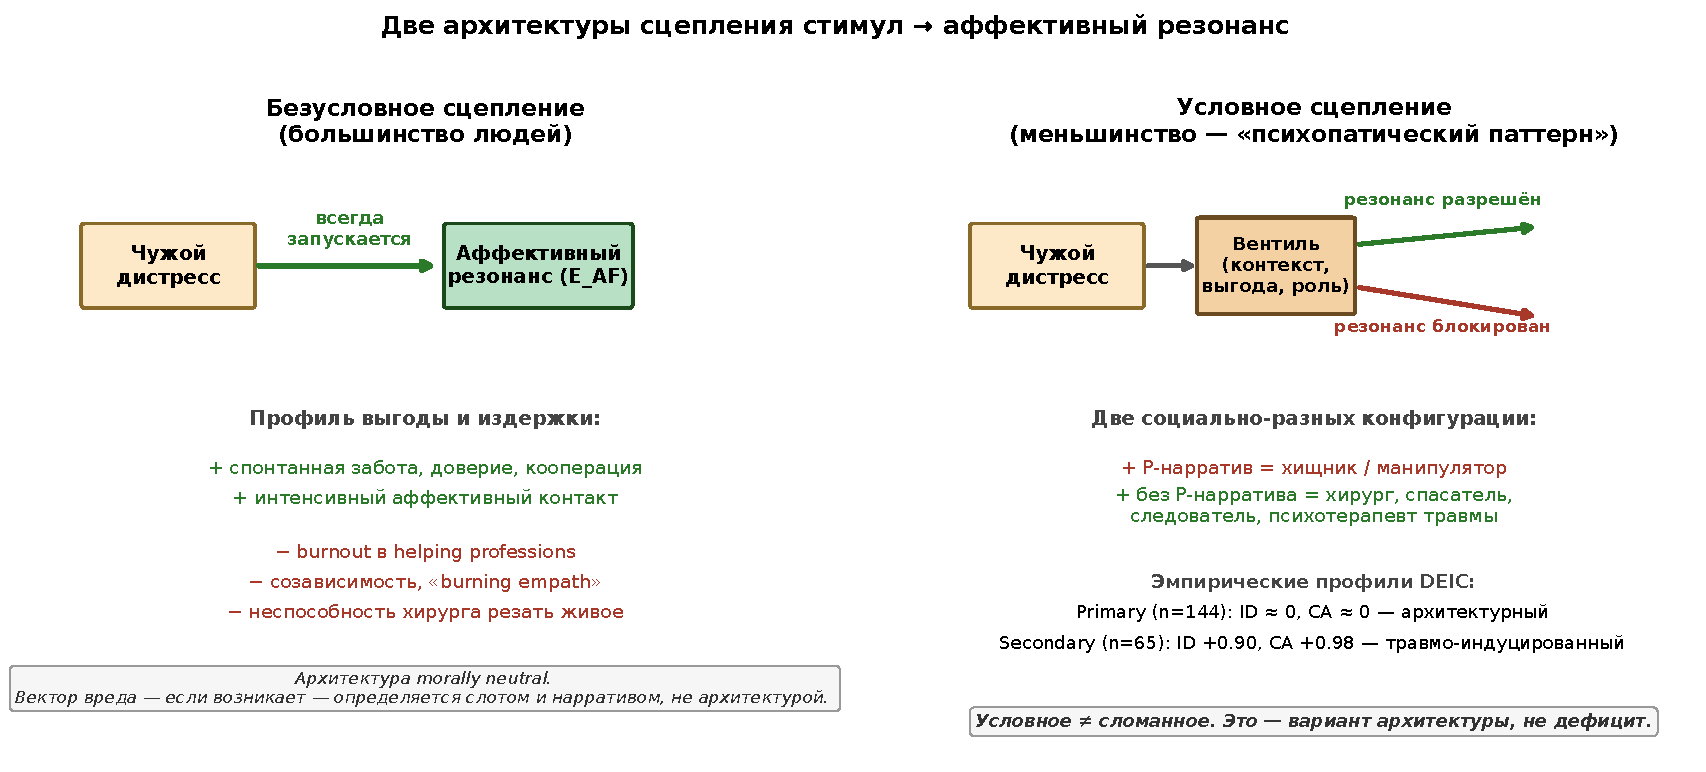
\includegraphics[width=0.95\linewidth]{figures/fig12_conditional_coupling.pdf}
\caption[Безусловное vs условное аффективное сцепление]{Архитектура сцепления \EAF{}, не дефицит. Слева: \emph{безусловное} сцепление --- аффективный резонанс запускается автоматически, почти непроизвольно, независимо от контекста и моральной оценки (базовый паттерн большинства популяции). Справа: \emph{условное} сцепление --- тот же резонанс доступен, но пропускается через контекст-зависимый gate; комбинации этой архитектуры с P-нарративом определяют социальное применение. Эмпирические профили первичной ($n = 144$; ID $\approx 0$, CA $\approx 0$) и вторичной ($n = 65$; ID $=+0.90$, CA $=+0.98$) клеток показаны как две этиологические траектории в условную архитектуру.}
\label{fig:conditional_coupling}
\end{figure} Параллели в других функциональных системах помогают удерживать рамку без нормативного сноса: люди различаются по condition-sensitivity болевой реакции, по вегетативной реактивности, по дефолтному уровню arousal. Ни одна из этих вариаций не называется поломкой по умолчанию --- каждая оценивается в конкретном контексте применения.

Условное сцепление имеет важное двойное использование, которое обычно вытесняется из клинической рамки. В социальных ролях, требующих работы внутри ситуаций страдания \emph{без} автоматического аффективного entrainment, условная архитектура --- не только совместима, но и функционально необходима. Хирург, который во время операции способен оставаться когнитивно точным при работе с живой плотью и кровью пациента. Спасательный врач, который эффективен в катастрофе именно потому, что его аффективный резонанс не парализует его действий. Следователь, работающий с показаниями жертв сексуального насилия. Психотерапевт травмы, выдерживающий многолетний поток клиентских состояний без выгорания. Каждая из этих ролей требует \emph{условного} доступа к аффективному резонансу --- способности включить и выключить резонансную сцепку сознательно. Безусловная архитектура в этих ролях даёт высокую burnout-vulnerability; условная --- устойчивость. В популяционном масштабе эта вариация обслуживает функции, которые иначе общество не могло бы заполнить.

Вредной эта архитектура становится только в сочетании с \textbf{P-нарративом} --- устойчивым моральным утверждением «мне это разрешено», которое разворачивает условную сцепку в сторону преднамеренного использования других без моральной обязанности. Именно поэтому \DEIC{} моделирует P \emph{отдельно} от \EAF{}: аффективная архитектура сама по себе морально нейтральна, а моральный нарратив --- ортогональный слой, определяющий её социальное применение. Условная сцепка без P-нарратива --- хирург; условная сцепка с P-нарративом --- хищник. Безусловная сцепка с P-нарративом --- маловероятная комбинация, которая в данных встречается редко; безусловная сцепка без P-нарратива --- базовый эмпатический паттерн большинства популяции, с его собственными уязвимостями.

В наших данных эта двухслойная логика хорошо видна в трёх эмпирических результатах. Первый --- \textbf{параллельная медиация CA $\to$ \{ID, P, M\} $\to$ \EAF{}} на единой модели (§\ref{sec:results}.4.1): путь CA $\to$ P по сути пуст ($a$-коэффициент $+0.015$, indirect effect 95\% CI $[-0.086, +0.060]$ включает ноль), в то время как путь через ID несёт $\sim 173\%$ тотального эффекта CA на \EAF{}. На уровне популяции P и CA статистически ортогональны. Это значит, что P-нарратив --- \emph{не} адаптивное следствие детской истории, а архитектурно независимый слой. Вторичный (hi-P-hi-CA) паттерн --- не «P через CA», а co-occurrence двух независимых осей в подгруппе людей. Первичный (hi-P-lo-CA) паттерн соответственно не является «психопатией без травмы в детстве», он вообще не принадлежит к той же этиологической линии, что CA-опосредованные конструкты.

Результат параллельной медиации требует честной реконсиляции с unified SEM (§\ref{sec:results}.4.2), где все пути --- параллельные медиаторы, A main-effect на \EAF{}, и модерация A на обеих стадиях ID-канала --- оцениваются одновременно. В этой более полной спецификации $a$-путь CA$\to$ID остаётся устойчивым ($+0.345$), CA$\to$P по-прежнему пуст ($+0.011$, NS), но $b$-путь ID$\to$\EAF{} коллапсирует до $-0.012$ (NS) при включении P в то же уравнение, тогда как P$\to$\EAF{} доминирует на уровне $-0.726$. Индекс модерации \IMM{}, значимый в более узкой спецификации §\ref{sec:results}.4 ($-0.00197$, CI не включает ноль), также коллапсирует до $+0.0001$ (NS), когда в той же модели P и A присутствуют как предикторы \EAF{}. Это не опровержение §\ref{sec:results}.4 и не артефакт переподгонки --- это ре-композиция дисперсии. В популяционном масштабе основная объяснительная сила \EAF{} концентрируется в P-канале (нарратив «разрешено мне») и в A-main-effect (witnessing как самостоятельный позитивный предиктор \EAF{}, $b = +0.393$), а не в изолированной ID$\times$A-модерации. На клиническом case-level каскад CA $\to$ ID $\to$ снижение \EAF{} остаётся содержательно значим --- $a$-путь реален, ID как медиатор травматического опыта в индивидуальной динамике присутствует; однако когда мы смотрим на общую выборку, прямой негативный предиктор аффективной эмпатии --- не остаточный ID, а активный P-нарратив и (в обратную сторону) активное witnessing-присутствие.

Это уточнение важно, потому что оно меняет клинико-теоретическую формулировку без потери основного содержания. Мы не утверждаем, что ID-канал отсутствует. Мы утверждаем: на уровне всей популяции ID-канал и P-канал имеют значительную общую дисперсию в предсказании \EAF{}, и в unified-модели основной вес несёт P (с его моральной подписью) и A (с его witnessing-слоем). Этот результат усиливает, а не ослабляет тезис §\ref{subsec:architecture} о двухслойной архитектуре: архитектурный уровень (условная/безусловная сцепка) и нарративный уровень (P-разрешение) работают \emph{независимо} от детской истории --- и их комбинация определяет социальное применение эмпатии куда сильнее, чем остаточный диссонанс ID сам по себе. ID --- важный индикатор того, \emph{что происходит} внутри травмированной психики; P --- решающий предиктор того, \emph{во что эта архитектура разворачивается} на поведенческом выходе.

Второй --- разделение первичного и вторичного паттернов. Через rule-based $2\times 2$ топологическую классификацию мы выделяем \textbf{первичный паттерн} ($n = 144$): условная сцепка без травматической истории, с выраженным P-нарративом, без внутреннего конфликта (ID $\approx 0$, CA $\approx 0$). Это конфигурация, стабильная во времени, не требующая травматического источника --- архитектурная вариация, на которую P-нарратив «надстраивается» как самостоятельная моральная структура \citep[в терминах][эмпирически --- в подобных пропорциях у \citealp{lilienfeld1990, patrick2010}]{karpman1941}. \textbf{Вторичный паттерн} ($n = 65$): условная сцепка с травматической историей (CA $= +0.98$), с активным внутренним конфликтом (ID $= +0.90$), с высоким Masking ($+0.63$). Это конфигурация, в которой условный режим сцепления функционально \emph{вынужден} защитной системой: автоматическое аффективное entrainment было бы разрушительно, и психика выстроила условное сцепление как адаптацию. P-нарратив здесь обычно остаётся активным, но структурно отличается --- он защищает остатки self, а не открывает доступ к хищничеству.

Третий результат --- распределение A-фактора (внимания) между группами и его взаимодействие с архитектурой. Первичный паттерн имеет умеренный A без особых корреляций с ID. Вторичный паттерн имеет низкий A ($-0.55$) --- его условная сцепка работает \emph{без} наблюдающего отношения, что делает её болезненной для самого носителя. Это прямо указывает на разные клинические точки входа: первичный паттерн не имеет «раны», которую можно лечить, и работа с ним --- структурно-социальная и нарративная (ограничение P-нарратива через внешние рамки, если это уместно); вторичный паттерн имеет «рану» в виде сохранного ID, и A-work переводит условное сцепление в интегрированный режим --- тот же профиль, что у интегрированного выжившего из §\ref{subsec:integrated_survivor}, но пришедший из другой истории.

Это не воспроизведение \emph{таксона} по \citet{hare2003} и не утверждение, что первичный и вторичный --- разные биологические виды. Мы утверждаем более скромное: архитектура условного сцепления в популяции существует как стабильная вариация, этиологически она достигается как минимум двумя путями (без травмы --- первичный; через травму как адаптация --- вторичный), и клиническая интерпретация «психопатия» смешивает эти пути, потому что на поведенческом уровне они выглядят похоже. Различить их можно только через измерение ID и CA. Без этого различия терапевтические стратегии систематически ошибаются: применение травма-ориентированных методик к первичному паттерну попадает в пустоту; применение поведенческих ограничительных методик к вторичному --- игнорирует его внутренний конфликт и потенциальный ресурс.

Размер вторичной подгруппы ($n = 65$) не позволяет надёжно оценивать величины эффектов; это ограничение требует клинической выборки для подтверждения. Но направление различения устойчиво воспроизводится в латентной топологии и не является артефактом одного индекса.

\paragraph{Возрастная инвариантность и критическое окно формирования архитектуры.} Анализ возрастной стратификации даёт один из наиболее клинически содержательных результатов программы: структурные связи между переменными --- центральный канал CA$\to$ID$\to$\EAF{}, ортогональность CA$\perp$P, ассоциации A с \EAF{} --- инвариантны в диапазоне возрастов 14--45 лет. Полная инвариантность в этом диапазоне значит, что архитектура, измеренная в наших данных, после \emph{раннего детства} структурно стабильна. Она может меняться в интенсивности (ID может ослабляться в результате терапии, A может расти в результате практики), но не в своей топологии: каналы, по которым проходит ущерб, и узлы, в которых он компенсируется, --- те же в 14 лет, те же в 45. Это указывает на то, что \textbf{критическое окно формирования архитектуры закрывается до 14 лет, и почти наверняка существенно раньше}. Нейродевелопментальная литература \citep{schore2001, perry2002, siegel2012} устойчиво указывает на первые 3--5 лет жизни как на период, в котором формируются базовые паттерны аффективной регуляции и attachment-архитектуры; наш результат совместим с этой датировкой и не противоречит ей. Практическое следствие --- структурная переформулировка prevention: если архитектура устанавливается до возраста, в котором типичный клиент попадает к клиницисту или в систему mental healthcare, то \emph{вся взрослая терапевтическая работа} --- это работа с уже сложившейся структурой, а не её первичное формирование. Рычаг первичной профилактики находится на уровне родительско-детского поля в первые годы жизни --- в поддержке mentalization-capacity родителей, в институтах раннего вмешательства, в dyadic parent-infant интервенциях \citep{powell2013}. В координатах \DEIC{} это не риторический призыв, а прямое операциональное следствие: ни одна из наших интервенционных гипотез (somatic work, MDMA-PT, psychedelic-assisted therapy, A-training) \emph{не создаёт} новую архитектуру у взрослого клиента; они все перестраивают существующую. Создание происходит до того, как клиент оказывается в состоянии обратиться за помощью.

Эта переформулировка --- архитектура вместо дефицита --- имеет последствия за пределами клиники. В уголовно-правовой системе, где психопатия часто трактуется как сочетание моральной и функциональной неисправности, разделение архитектуры (нейтральной) и P-нарратива (морально значимого) разводит то, что требует коррекции, от того, что не подлежит коррекции в принципе (архитектуру). В организационной психологии разделение позволяет видеть, что некоторые роли нуждаются в условной архитектуре и что её «лечение» противоречит функции. В публичной коммуникации --- позволяет перестать говорить о психопатах как о «сломанных людях» и перейти к разговору о комбинации способностей и нарративов, который социум может регулировать через внешние структуры, а не через попытку переделать внутреннюю архитектуру.

\subsection{Позиционирование: слон, а не мастер-карта}
\label{subsec:positioning}

Мы сознательно выбираем позиционирование, которое отличается от большинства интегративных психологических проектов. \DEIC{} не претендует быть «первым единым фреймворком эмпатии», «разрешением дискуссии между психоанализом и нейронаукой», «интеграцией всех традиций». Мы выбираем более узкую и более защитимую позицию: \DEIC{} --- это \emph{компрессия}, а не \emph{сложение}. Разные традиции (психоаналитическая, теория привязанности, когнитивная нейронаука эмпатии, зеркально-нейронная литература, клиническая традиция психопатии от Cleckley к Hare, контемплативные традиции witnessing) действительно касаются одного и того же предмета разными способами, и каждое касание --- настоящее. Наш вклад в том, что мы измерили шесть различимых функций в \emph{одной} выборке, показали их устойчивые структурные отношения и тем самым сделали видимыми \emph{суставы} между тем, что эти традиции описывают по отдельности.

Мы специально не занимаем позицию, которую \citet{wilber1995, wilber2000} занимал по отношению к традициям. Уилбер утверждал, что существует \emph{супер-карта} (AQAL: четыре сектора $\times$ уровни $\times$ линии $\times$ состояния $\times$ типы), на которой каждая традиция занимает своё иерархически определённое место. Это онтологическая претензия: карта первична, традиции вторичны, и каждая видит лишь фрагмент того целого, которое видит мета-теоретик. В нашей работе четыре реальных отличия от этой позиции важны и будут соблюдены как дисциплина, а не как стилистика.

Во-первых, уровень претензии. Уилбер строит онтологию --- мета-метафизическое утверждение о том, как устроена реальность. \DEIC{} строит measurement model --- психометрическую модель шести функций на конкретной выборке. Первое неопровержимо по конструкции; второе должно воспроизводиться в новых выборках, и если не воспроизводится, оно опровергнуто.

Во-вторых, иерархия координат. В AQAL уровни иерархичны и нормативны: integral $>$ pluralistic $>$ rational $>$ mythic $>$ magical $>$ archaic. В \DEIC{} шесть координат не иерархичны. Нет предустановленной позиции, что «высокое A лучше» или «низкое P лучше»; есть эмпирические корреляции с исходами, но это следствия данных, а не нормативные оценки. «Интегрированный выживший» --- один профиль среди многих, а не вершина.

В-третьих, отношение к традициям. Уилбер ассимилирует: каждая традиция получает место на \emph{его} карте, и её внутренняя структура переинтерпретируется через AQAL. \DEIC{} не размещает традиции. Мы говорим: «измеренный нами конструкт X коррелирует с тем, что в традиции A называют \textit{sākṣī}, в традиции B --- \textit{rigpa}, в традиции C --- самовоспоминание». Эти описания в своих системах автономны. Мы не встраиваем системы в \DEIC{}; мы показываем, где психометрическая координата \emph{нашей} модели коррелирует с тем, что описывают они.

В-четвёртых, скромность относительно непонятого. Уилбер объясняет всё, включая внутренние противоречия --- они ассимилируются как «более низкий уровень смотрит на более высокий». \DEIC{} имеет эксплицитный список того, что он не объясняет (см. §\ref{sec:limitations}, §\ref{sec:future}): временной каркас, механизм переключения между ID и P, механизм терапевтической силы A, индивидуальные различия в A-trainability, developmental branching в $2\times 2$, эволюционно-экологическая подложка, рефлексивность наблюдателя. Это не дефект, это граница.

Короткая формула, которая будет повторяться в этом разделе несколько раз: Уилбер --- «я вижу целое; традиции видят части моей карты; вы сейчас на уровне X»; \DEIC{} --- «я вижу шесть измеримых функций. Некоторые традиции описывают одну из них глубже, чем мы. Координатный каркас --- не метафизика, а статистика; его можно и нужно опровергать».

\subsection{Дисциплина анти-Уилбер: гигиена языка}
\label{subsec:discipline}

Позиция из §\ref{subsec:positioning} реализуется через набор дисциплинарных правил, которые должны выполняться в каждом абзаце. Первое правило --- каждое утверждение о конструкте сопровождается фальсификатором. Если мы пишем «A модерирует канал CA$\to$ID$\to$\EAF{}», мы обязаны добавить: «если в pre-registered replication \IMM{} 95\% CI включает ноль, это утверждение опровергнуто». Этим мы отличаем \DEIC{} от систем, которые объясняют всё (и тем самым не объясняют ничего).

Второе --- запрет иерархии между факторами. Мы не пишем «A --- зрелость», «интегрированный выживший --- высшая точка», «witnessing --- более развитый уровень». Мы пишем «эмпирически связано с [конкретный результат]». Это может показаться педантизмом, но именно в этой точке большинство мета-теоретических проектов сходит с рельсов: нормативный язык встраивается незаметно и закрывает дорогу эмпирической проверке.

Третье --- не ассимилировать традиции, но и не держать их на символической дистанции. Мы не пишем «Дзен --- это про A». Мы пишем «Дзен описывает похожий конструкт в своей системе; корреляция с нашей моделью --- такая-то». Если мы не можем сделать вторую часть утверждения, мы не делаем и первую. При этом мы \emph{делаем} вторую часть --- и делаем её развёрнуто, когда традиция даёт операбельное различение, которое в психометрической литературе пока не воспроизведено. Культурологические референты (адвайта, дзогчен, Четвёртый путь, non-dual современность, Маккенна) в \DEIC{} --- не декоративное оформление и не проявление академической смелости в ущерб строгости; они источники гипотез, которые мы либо формулируем как фальсифицируемые, либо оставляем без упоминания. Байесовский приор при расхождении наших данных с контемплативной традицией --- «мы ещё не измерили то, что они различают», а не «они ошибались».

Четвёртое --- measurement model $\neq$ онтологические претензии. Мы не пишем «\DEIC{} описывает психику». Мы пишем «\DEIC{} --- психометрическая модель шести функций на $N = 1426$ русскоязычной онлайн-выборке». Это ограничение претензии, которое защищает нас от превращения в мета-теорию.

Пятое --- лексическая дисциплина. \emph{Extends, operationalizes, is consistent with, replicates within our framework, provides psychometric coordinates for} --- разрешено. \emph{Unifies, completes, first to integrate, resolves, supersedes, subsumes} --- запрещено. Выбор глагола в ключевом утверждении программы --- это выбор между серьёзной работой и мета-теоретической претенциозностью.

Шестое --- обязательная секция «что \DEIC{} не объясняет» видимого размера, не в сноске (см. §\ref{sec:limitations}--\ref{sec:future}).

Седьмое --- reflexivity clause: в методологической статье программы будет эксплицитный раздел о том, что наблюдатель (исследователь) со своим уровнем A влияет на то, что он способен измерить у наблюдаемого. Это структурное эпистемологическое признание, а не мистическая ремарка.

\subsection{Фальсифицируемость как структурный уровень}
\label{subsec:falsifiers}

Генеративный характер модели важнее её описательного характера. Все предсказания, сформулированные в предыдущих подразделах Обсуждения, --- двухстадийная A-модерация канала CA$\to$ID$\to$\EAF{}, коллапс $b$-пути ID$\to$\EAF{} в unified SEM, ортогональность CA$\perp$P на популяционном уровне, различимость первичной и вторичной психопатии, \EAF{}-эффект в интегрированно-выжившей клетке, hyper-instrumentation P$\to$\Ecog{} и прочие --- вынесены в отдельный структурный раздел (§\ref{sec:falsification}) в форме claim/falsifier-пар с явно указанными требованиями к тесту и последствиями опровержения. Тот раздел не является расширенным комментарием к Обсуждению; он формулирует, \emph{при каких именно наблюдениях} утверждения этой статьи следует считать ложными. Для чтения Обсуждения это означает: все утверждения в findings-регистре («данные показывают», «модель даёт») имеют научный статус ровно в той мере, в какой в §\ref{sec:falsification} сформулирован их фальсификатор. Этот раздел --- не приложение к статье, а условие того, что статья принадлежит к эмпирическому жанру, а не к риторическому.

\subsection{Отношение к существующим теориям}
\label{subsec:relation_to_theories}

\DEIC{} совместим с большинством основных линий эмпатии и психопатии, но в ряде точек не совпадает с доминирующими интерпретациями. Мы не заявляем, что эти линии ошибочны целиком; мы указываем точки, в которых наша модель расходится с ними.

\citet{baroncohen2011} EQ как диспозиционная черта --- в нашей модели \EAF{} --- state, регулируемый A; trait-модель пропускает ядро механизма. «Psychopaths lack cognitive empathy» --- популярное упрощение; наши partial correlations показывают обратное: $r$(P, \Ecog{}) $= +0.32$ после partialling. Когнитивная эмпатия у психопатов часто \emph{повышена}; именно это обеспечивает возможность «хищничества», как описано у \citet{blair2013} и \citet{baroncohen2011} под рубрикой hyper-instrumentation. Hare'овский таксон-взгляд на психопатию --- мы не находим categorical kinds в наших данных. Dimensional-модель с двумя ортогональными этиологиями точнее описывает топологию наших результатов. \citet{newman2003} response modulation theory как универсальное объяснение психопатии --- у наших P-паттернов когнитивное внимание сохранно; witnessing-аффективная сцепка работает в \emph{условном}, а не безусловном режиме. Ответно-модуляционное объяснение фиксирует часть этого механизма --- избирательность внимания, --- но не отделяет архитектурный слой (условное сцепление, морально нейтральное) от нарративного (P-разрешение).

Classic attachment determinism \citep{bowlby1969} в упрощённом прочтении: CA $\to$ dysfunction линейно. Наши данные показывают модерацию через A. Детерминизм ложен; компенсация эмпирически реальна. \citet{vaillant1977} иерархия зрелых/незрелых защит --- мы не находим, что защиты per se патологичны. ID без A даёт дисфункцию; ID с A --- функциональную компенсацию. Моральная рамка «зрелая защита лучше незрелой» оказывается менее информативной, чем рамка «защита плюс witnessing».

NICE/APA CBT-first для всех расстройств настроения \citep{nice2022, apa2019}. \DEIC{} прямо предсказывает, что у high-ID / low-A клиентов CBT попадёт в сопротивление или даст поверхностное улучшение без изменения базового механизма. Self-reported psychiatric dx count как severity measure --- наши данные показывают, что ID блокирует help-seeking, поэтому dx\_count \emph{недооценивает} самых тяжёлых случаев. FFMQ \citep{baer2006} как операционализация mindfulness --- наш A-CFA эмпирически демонстрирует, что метакогнитивные айтемы смешивают attention-to-internal-states с witnessing. Мы поддерживаем критику \citet{vandam2018}. \citet{wilber1995, wilber2000} AQAL --- мы прямо не воспроизводим иерархически-стадиальные модели развития сознания в наших данных. Мы не находим stages; мы находим дистрибутивные неиерархичные координаты.

\subsection{Расширение ACE: «не помню» как часть конструкта, а не пропуcк}
\label{subsec:ace_extension}

Стандартная операционализация adverse childhood experiences, идущая от \citet{felitti1998} и закреплённая в CDC/Kaiser-линии и практически во всём производном корпусе, допускает у респондента два легитимных ответа на каждый ACE-айтем: «да» (событие было) и «нет» (не было); всё остальное --- «не помню», «не уверен», отказ --- трактуется как missing data, исключается или импутируется. ACE-айтемы при этом спрашивают не об эмоциональной интерпретации детского опыта, а о \emph{фактах}: был ли родитель в заключении, употребляли ли в семье вещества, происходило ли домашнее насилие, умер ли родитель, развелись ли родители. На фактологический вопрос ответ «не помню» в популяционной перспективе имеет ровно две содержательные интерпретации, и \emph{ни одна из них не сводится к статистической missingness}. Первая: респонденту не рассказывали --- что само по себе является маркером семейного паттерна замалчивания вокруг высокоадверсивной среды (семьи, в которых систематически обсуждают умершего родителя или эпизод насилия, производят других респондентов, а не тех, кто отвечает «не помню»). Вторая: респондент диссоциировал --- что является прямой поведенческой манифестацией того самого защитного механизма D, который ID-латент измеряет на другом конце инструмента. Обе интерпретации ACE-релевантны; обе эмпирически противоположны трактовке «не помню» как missing. Стандартная кодировка в таком случае \emph{исключает из анализа ровно тот подконтингент, на котором ACE-сигнал должен быть наиболее силён}. Это не мелкая кодировочная деталь, а структурный недо-учёт в стандартной методологии ACE, наследованный всем корпусом.

DEIC-конструкт предлагает расширение: ответ «не помню» на ACE-айтеме следует трактовать как \emph{позитивный сигнал адверсивно-релевантной семейной или когнитивной конфигурации} --- либо семейного замалчивания, либо диссоциативного encoding-gap, --- и кодировать численно наравне с «да». Тогда ACE перестаёт быть одномерным счётчиком событий и становится двухслойным: явный счёт подтверждённых событий плюс счёт ответов «не помню» как отдельная ACE-dissociation подшкала.

Эмпирическая валидация расширения получена на текущей выборке через полный re-fit 6-факторной oblique CFA, в которой канонический код «не помню»~$=$~NaN заменён на «не помню»~$=$~1. Из 1470 респондентов 667 (45.4\%) использовали «не помню» хотя бы один раз на 10 ACE-айтемах; 294 (20\%) --- дважды и более. Под расширенной кодировкой N проходит фильтр $\le$10\% missing уже 1468 (против канонических 1426), средний ACE-счёт сдвигается с 3.43 до 4.18, MLR-robust CFA сохраняет приемлемый фит (CFI~$=$~0.960, TLI~$=$~0.949, RMSEA~$=$~0.062 против канонических 0.950, 0.936, 0.068; df~$=$~120 в обоих случаях). Латентные корреляции в 6-факторной oblique модели сдвигаются в направлении, согласующемся с DEIC-гипотезой: $r(\text{CA}, \text{ID})$ растёт с $+0.668$ до $+0.712$, $r(\text{CA}, \EAF{})$ усиливается по модулю с $-0.129$ до $-0.205$ ($+59\%$), $r(\text{CA}, M)$ растёт с $+0.195$ до $+0.267$, тогда как $r(\text{CA}, P)$ остаётся слабой (рост с $+0.015$ до $+0.122$ --- всё равно в пределах «слабой» связи), сохраняя архитектурную орто\-гональность P к детской адверсии.

Параллельная медиация CA~$\to\{$ID, $P$, $M\}\to\EAF{}$ на латентных scores split-B под канонической и расширенной кодировкой (5000 bootstrap-draw) даёт согласованно усиленную картину. Суммарный эффект $c$(CA~$\to$~\EAF{}) усиливается по модулю с $-0.129$ до $-0.205$. Косвенный эффект через ID --- канонический канал «защита убивает эмпатию» --- сохраняет структуру: $-0.223$ [$-0.267, -0.181$] под канонической кодировкой, $-0.236$ [$-0.282, -0.192$] под расширенной; CI в обоих случаях не пересекает ноль. Косвенный эффект через P \emph{становится статистически отличимым от нуля} именно при расширении: канонический $-0.014$ [$-0.086, +0.060$] (нз), расширенный $-0.140$ [$-0.234, -0.048$] (стат.~значимый). Это не переопределяет архитектурную орто\-гональность P к CA как популяционный факт, но указывает, что часть P-канала была инструментально недо-замечена именно там, где у респондента включена диссоциативная кодировка детства. Прямой эффект $c'$ (CA~$\to$~\EAF{} при контроле ID, P, M) остаётся положительным при обеих кодировках ($+0.073$ канонический, $+0.048$ расширенный), то есть headline sign-flip главного mediation-вывода --- «травма бьёт по эмпатии через защиту, а не напрямую» --- устойчив к способу кодировки «не помню». Ни один из 95\%-ных bootstrap-интервалов для исходных статзначимых индиректов не пересекает ноль под расширенной кодировкой, то есть сдвиги численно различимы, а не шумовые.

Операциональное следствие для волны 2: ACE-айтемы сохраняют трёхвариантный формат «да / нет / не помню», но «не помню» кодируется как позитивный сигнал; счётчик таких ответов по всем 10 айтемам строится как самостоятельная ACE-dissociation подшкала. Психометрическое предсказание: при $n \ge 300$ эта подшкала должна давать McDonald's $\omega \ge 0.7$ и положительно коррелировать с ID-латентом ($r \ge 0.30$ при латентном оценивании); при её контроле связь «явного» ACE-счёта с ID должна ослабевать, что даёт формальный тест валидности подшкалы как отдельного канала. Концептуальное следствие шире. Мы не утверждаем обобщение \emph{эффект-сайзов} на весь корпус ACE-литературы --- для этого нужен мета-аналитический re-фит; мы указываем на \emph{структурную} проблему в кодировочной логике, наследованной всем корпусом \citep{felitti1998}. Там, где эта логика одинакова, одинаков и направленный смыслостроительный сдвиг: любой self-report сенситивной информации ранних лет жизни --- сексуального анамнеза, substance-history, семейных секретов --- где «не помню» является легитимным и социально-приемлемым ответом, требует явного моделирования этого ответа как construct-relevant signal, а не механического сведения к missing. См. §\ref{sec:future} о дизайне wave-2 и §\ref{sec:limitations} о границах текущей оценки.

\subsection{Декларативно-поведенческая асимметрия (DI) как сигнал архитектурной фрагментации}
\label{subsec:di_asymmetry}

Пилотная композитная версия инструмента (DEIC-DRAFT, август 2025) была построена на принципе парных формулировок: каждый содержательный айтем существовал в декларативном регистре (абстрактная self-description: «я эмпатичный человек», «я манипулирую другими», «я подавляю свои эмоции») и поведенческом регистре (конкретная узкоокнская поведенческая репортация: «вчера я остановился и действительно выслушал», «на прошлой неделе я скрыл от партнёра важную деталь ради своей выгоды», «сегодня утром я сдержался от того, чтобы показать раздражение»). Сводный индекс $DI = \overline{\text{decl}} - \overline{\text{beh}}$ по всем айтемам в пилоте показал статистически значимый популяционный сдвиг ($p < 0.001$, $d \approx 0.43$) с ведущим вкладом шкалы AIS (декларативно 5.04 vs поведенчески 3.35). На этом основании в пилотном отчёте DI был описан как самостоятельный индикатор social desirability. Ниже мы показываем, что это описание было частично неверным: популяционный сдвиг воспроизводится, но по шкалам он разнонаправлен, и то, что DI на самом деле измеряет --- не однородное искажение самопрезентации, а \emph{архитектурный разрыв между абстрактным self-schema и эпизодической поведенческой памятью}.

На основной выборке ($N{=}1470$) декларативно-поведенческий разрыв посчитан по восьми шкалам с достаточным балансом парных айтемов (ADI, CA, D, EC, Empathy, Psychopathy, Suppression, Masking; 38 декларативных против 40 поведенческих). Парные $t$-тесты значимы на всех восьми шкалах, но распределение $d$ по модулю и направлению существенно различается. Положительные DI (декларация превышает поведение) --- E ($d{=}{+}0.44$), EC ($d{=}{+}0.45$), ADI ($d{=}{+}0.20$), CA ($d{=}{+}0.19$). Отрицательные DI (поведение превышает декларацию) --- P ($d{=}{-}1.05$; крупнейший эффект на выборке), MS ($d{=}{-}0.30$), S ($d{=}{-}0.10$), D ($d{=}{-}0.09$). Суммарный сырой DI оказывается слабо отрицательным ($d{=}{-}0.11$) --- знак усреднения разнонаправленных шкал. Если же DI выровнять в prosocial-направлении (для стигматизированных шкал знак перевернуть, так чтобы $+$ всегда означало «я декларативно прохожу как более положительная версия себя, чем показывает моё поведение»), сдвиг становится однородно положительным: $d_{aligned}{=}{+}0.29$, 95\%CI $[{+}0.14, {+}0.20]$. Пилотное наблюдение, таким образом, воспроизводится, но как \emph{совокупный результат двух разных механизмов}, а не однородный social-desirability bias.

Разведение этих механизмов --- главный содержательный результат этого раздела. Для стигматизированных шкал с явным self-incriminating содержанием (P, MS, S, D) поведенческие айтемы узкой фокусировки («на этой неделе я...») собирают больше признаний, чем декларативные trait-описания, --- то, что респондент не готов присвоить как черту, он готов признать как эпизод. Наиболее ярко это проявляется на P: пара $P_4$ («я манипулирую людьми, чтобы получить желаемое») --- $P_{\text{new\_3}}$ (конкретное поведенческое описание эксплуатационной ситуации за прошедший период) даёт средний разрыв $-2.66$ балла по 7-балльной шкале ($d{=}{-}0.98$), то есть respondent систематически отрицает trait-схему психопатии, но отчётливо опознаёт конкретные её проявления в собственном поведенческом архиве. Это воспроизводит давнее клиническое наблюдение о расщеплении между trait-идентификацией и эпизодическим поведенческим self-report при психопатическом нарративе \citep{hare2003, lilienfeld1990} на операциональном уровне. Для desirable-валентных шкал (E и, с оговоркой, EC) направление противоположно: trait-schema широка, поведенческий эпизод узок --- respondent держит развитое самопредставление об эмпатичности, которое опирается на широкую историю, в то время как конкретный narrow-window beh-айтем («сегодня утром я \ldots») попадает или не попадает в конкретный поведенческий эпизод. Для shared-adversity шкал (ADI, CA) положительный разрыв указывает на противоположный паттерн: trait-уровень отчасти overstates внутреннюю историю, которой конкретный поведенческий эпизод в повседневности не подтверждает --- возможное методологическое следствие того, что ADI- и CA-декларативные айтемы опрашивают глобальный аффективный self-concept, не привязанный к недавнему коду.

То, что DI не сводится к social desirability, подтверждается связями с латентной архитектурой. $DI_{overall}$ (сырой, ненаправленный) коррелирует с ID как $r{=}{+}0.590$, с CA как $r{=}{+}0.580$ и с A как $r{=}{-}0.517$; с клинической диагностической переменной ($\text{dx\_free\_text\_any}$) --- $r{=}{+}0.017$ (нз, $p{=}0.66$). Иначе говоря, величина декларативно-поведенческого разрыва отслеживает \emph{внутреннюю фрагментацию между слоем trait-self-schema и слоем episodic-behavior-recall}, и эта фрагментация маркирована тем же архитектурным латентом (ID), который во всей остальной работе фиксируется как защитный контур. $A$ как witnessing-функция сужает разрыв. Клинический статус в этом не участвует, что структурно последовательно с $\S\ref{subsec:architecture}$ и $\S\ref{subsec:free_will}$: DI --- архитектурная, а не диагностическая метрика. $DI_{aligned}$ (развёрнутый в prosocial-направлении) даёт зеркальную картину: $r(DI_{aligned}, A){=}{+}0.658$, $r(DI_{aligned}, \EAF{}){=}{+}0.550$, $r(DI_{aligned}, ID){=}{-}0.645$, $r(DI_{aligned}, P){=}{-}0.362$. При медианном расщеплении по $A$ контраст $DI_{overall}$ между low-A и high-A даёт $d{=}0.90$ (терцильный --- $d{=}1.22$), то есть $A$-поле полностью перестраивает направление и величину разрыва.

Отдельный результат касается $piz$ --- интегральной метрики, реализованной в инструменте для отслеживания фасадной работы (masking+Lie; $\S\ref{subsec:integral_metrics}$). $piz$ и DI структурно различны и эмпирически различны. $r(piz, DI_{overall}){=}{+}0.198$ (small positive), $r(piz, DI_{aligned}){=}{-}0.274$ --- то есть $piz$ и $DI_{aligned}$ даже расходятся по знаку (более высокое маскирование $\Rightarrow$ \emph{меньший}, а не больший prosocial-сдвиг декларации над поведением). На отдельных шкалах $r(piz, DI_{P\_scale}){=}{+}0.359$: более высокое маскирование связано с более выраженным $\textit{beh}>\textit{decl}$ разрывом на P-шкале (высокая facade-работа усиливает именно ту ассиметрию, при которой trait-отрицание идёт рука об руку с поведенческим признанием). В сумме: $piz$ измеряет самопрезентационное давление, $DI$ измеряет структурную фрагментацию --- два разных слоя, оба операционализуемы.

Для инструментальной инфраструктуры это означает, что $DI$ имеет смысл фиксировать рядом с $piz$ как шестую \texttt{extended\_metric} в \texttt{psychometrics.json} (с per-scale и overall-aligned версиями). Для теоретической рамки --- что пилотное наблюдение восстанавливается, но в содержательно уточнённом статусе: оно даёт операциональную psychometric-сетку для давнего психоаналитического различения между «идеальным Я» как trait-schema и «действующим Я» как поведенческим архивом \citep{freud1917, winnicott1965}, при этом разрыв между ними --- не дефект измерения, а содержательный маркер архитектуры. Методологическое следствие для wave-2: любая психометрическая шкала, претендующая на диагностическую функцию в $ID$/$P$/$E$-доменах, должна включать парные декларативные и поведенческие формулировки, потому что именно их разрыв, а не любая из двух формулировок по отдельности, даёт доступ к архитектурному слою.

\subsection{\DEIC{} и теория сознания: граница, на которой мы работаем}
\label{subsec:consciousness}

\DEIC{} не предлагает теорию сознания. Hard problem \citep{chalmers1995} --- граница, через которую психометрия не проходит и не должна делать вид, что прошла. Мы измеряем функции \emph{внутри} сознания (внимание, диссонанс, эмпатия); мы не утверждаем ничего о природе субъективного опыта как такового, и это ограничение серьёзное, а не риторическое.

Но из того, что граница реальна, не следует, что от неё нужно держаться на дистанции. Наоборот: именно вблизи этой границы происходит самый содержательный интерфейс эмпирической психометрии с contemplative studies. A --- психометрический след того, что в различных традициях выделяется как структурно иной слой сознания: \textit{sākṣī} в адвайте, \textit{rigpa} в дзогчене, «самовоспоминание» у Гурджиева, non-dual awareness в современной non-dual литературе. Мы не объясняем, что такое свидетель. Мы показываем, что witnessing измеримо, функционально, и что его действие на канал CA$\to$ID$\to$\EAF{} воспроизводимо в узкой спецификации. Это делает A точкой, в которой психометрия \emph{соприкасается} с разделом сознания, который обычно считается вне-функциональным, --- не ассимилируя его и не заявляя о его природе, но и не обходя его стороной.

Самый резкий диалог этого типа --- с \citet{mckenna2002, mckenna2004, mckenna2013}. В большинстве западных репрезентаций contemplative traditions пробуждение описывается аддитивно: больше осознанности, больше принятия, больше присутствия. McKenna это переворачивает. Его тезис --- \emph{spiritual autolysis}: пробуждение есть разрушительный процесс, растворение иллюзорных структур, а не наращивание новых способностей. Больше внимания не приносит утешения; оно раскрывает сконструированность собственных состояний и мира, и это раскрытие не приятно. Обычный человек уклоняется от него, потому что там нет утешительной рамки.

В рамке \DEIC{} тезис McKenna формулируется как прямое longitudinal-предсказание. У людей, проходящих intensive retreats с глубокой witnessing-практикой, A растёт. Если McKenna прав, на коротком промежутке времени ID \emph{возрастает} --- раскрытие сконструированности даёт временную дестабилизацию identity, то есть именно ту сигнатуру, которую в нашей cross-sectional модели мы читаем как диссонанс. Траектория после этого разветвляется: либо регрессия (защиты возвращаются, A падает обратно, дестабилизация закрывается обычной структурой), либо интеграция (принятие сконструированности, профиль, топологически соответствующий integrated survivor из §\ref{subsec:integrated_survivor}, но пришедший не через детскую травму, а через добровольный практический путь). Это не предсказание «верный ли McKenna»; это операционализация его тезиса в виде, который может быть опровергнут longitudinal-данными на retreat-когортах.

Это и есть наше положение относительно теории сознания. Не заменять её, не претендовать на её территорию --- но и не делать из её существования предлог, чтобы избегать контакта. На границе работать можно и нужно: делать конкретные психометрические предсказания в тех точках, где contemplative traditions удерживают операбельные различения, которые эмпирическая психология пока только начинает уловить.

\subsection{Клинические импликации}
\label{subsec:clinical}

Модель имеет несколько конкретных клинических следствий, которые мы формулируем как \emph{предложения для тестирования}, а не как рекомендации к немедленному внедрению.

\paragraph{Работа с A до работы с содержанием.} У клиентов с высоким ID и низким A прямая когнитивная интервенция часто попадает в сопротивление или даёт поверхностное улучшение. Наша модель предсказывает, что последовательность «A-work $\to$ content-work» будет эффективнее, чем «content-work без предварительного A». Это формализует то, что somatic experiencing \citep{levine2015}, sensorimotor psychotherapy \citep{ogden2006}, IFS \citep{schwartz1995}, mentalization-based therapy \citep{fonagy2008} и ряд психодинамических подходов делают интуитивно. Pre-registered RCT с baseline A и ID как модератором эффекта лечения --- прямой тест.

\paragraph{Различение первичного и вторичного паттернов в клинической оценке.} Без измерения ID и CA два паттерна выглядят одинаково, но требуют разных стратегий. Первичный --- условная архитектура без «раны»: клиническая работа с архитектурой как таковой бесполезна и даже может быть неуместной (в функциональных социальных слотах эта архитектура даёт устойчивость); работа с P-нарративом через внешние рамки --- адекватна тогда, когда нарратив разворачивается в хищническую сторону. Вторичный --- работа с травмой и расширение A, с целью перевода сохранного ID в интегрированный режим.

\paragraph{A-training как центральный компонент долгосрочной работы.} Наша модель предсказывает, что non-dual mindfulness практика будет давать более сильный эффект на \EAF{}-восстановление, чем behavioral-mindfulness в стиле MBSR. Это формулирует head-to-head testable сравнение.

\paragraph{Burning empath как feed-forward риск.} Профиль CA + hi \EAF{} + lo A должен предсказывать burnout в helping professions.

\paragraph{Substance use как phenotype, не причина.} В подгруппе blocked-sober-high-P наблюдается тот же профиль P/D/ACE, что и у активных пользователей веществ. Это указывает, что substance --- \emph{выход} блокировки, а не её источник. A-training в работе с addictive behaviors должен давать устойчивый эффект там, где abstinence-based программы рецидивируют.

\paragraph{Терапевт с низким A не видит ID-активации клиента.} Это имеет прямое клиническое следствие: supervision и self-work клинициста --- не nice-to-have, а структурное условие возможности видеть то, что у клиента происходит.

\subsection{Свобода воли как градиент внимания}
\label{subsec:free_will}

Одно из наиболее концептуально тяжёлых следствий \DEIC{} --- реформулировка проблемы свободы воли. Мы не претендуем её решить. Мы утверждаем, что в её классическом бинарном виде --- «свободна ли воля?» --- она поставлена в неверной зернистости и потому не имеет ответа. В зернистости, которую даёт наша модель, она распадается на конкретный эмпирический вопрос: \emph{какова величина A в конкретной ситуации у конкретного агента?}

В DEIC-координатах поведение можно читать как результат взаимодействия двух слоёв: автоматической D/P/E-конфигурации (что запускается как ответ на стимул без участия наблюдающего отношения) и A (зазор между запуском и действием, в котором возможно иное распределение внимания, иное соотнесение, иная реакция). Low-A-агент в конкретный момент функционально детерминирован своей конфигурацией: стимул активирует канал, канал разворачивает автоматическое поведение, наблюдение отсутствует. High-A-агент в том же моменте имеет \emph{измеримый зазор} между активацией и действием, внутри которого возможна иная траектория. Это не метафизическое различие, а эмпирическая переменная --- та же, которую фиксирует наша A-модерация в узкой спецификации: при высоком A канал CA$\to$ID$\to$\EAF{} меняет знак именно потому, что A вклинивается между привычным триггером и его привычным исходом.

Философы, спрашивавшие о свободе воли, подходили к одному и тому же градиенту с разных сторон. Августиново «раб воли» и его описание \textit{liberum arbitrium captivatum} есть описание low-A состояния, в котором желание непрерывно разворачивается в действие без зазора. Кант и его примат практического разума --- описание функции, которая появляется при высокой A: \emph{Maxime} как осознаваемый принцип поведения, а не импульс. \citet{libet1985} с его ранней готовностной потенциалом и критики его интерпретации \citep[см.][]{frith2008} указывают на то, что волевой акт действительно иногда запаздывает относительно мозговой активности, но \emph{veto-функция} остаётся --- это и есть A, удерживающая зазор. \citet{frankl1946} --- «между стимулом и ответом есть пространство; в этом пространстве наша сила выбирать наш ответ» --- прямое описание A-модерации в клиническом языке. Буддистская \textit{vīmaṃsā} (исследующее внимание) и \textit{yoniso manasikāra} (обдуманное внимание) описывают практики, наращивающие A как условие этической возможности; адвайтическое различение \textit{vṛtti} (движения ума) и \textit{sākṣī} (наблюдающего) --- ту же самую структурную асимметрию. Гурджиевское «человек-машина» есть описание low-A-режима, а «самовоспоминание» --- операциональный протокол подъёма A. Когда эти линии сходятся на том, что обычный человек большую часть времени действует из автоматизма, а моменты свободы связаны с особым качеством внимания, они сходятся не случайно --- они описывают одно и то же измеримое явление в разных языках.

Из этого прочтения следует серия предсказаний. Во-первых, восприятие агенсом собственного волевого акта как «свободного» должно коррелировать с его моментальным A, а не с его trait-уровнем самоэффективности или с нарративом самодетерминации. \citet{westgate2019}-type парадигмы meaning-in-action могут быть переформатированы как A-assays. Во-вторых, интервенции, повышающие A (non-dual mindfulness, somatic work, psychedelic integration), должны давать измеримый рост переменных, которые обычно связываются с self-determination: внутренняя мотивация, моральная консистентность, способность отказаться от краткосрочного вознаграждения в пользу долгосрочной ценности. В-третьих, популяции с систематически подавленным A (см. §\ref{subsec:political}) должны демонстрировать систематически меньшую функциональную свободу выбора --- не как моральный дефект, а как прямое следствие разрушения операциональной инфраструктуры свободы.

Этическое следствие этого прочтения --- не отмена ответственности, а её структурная перекалибровка. Вопрос «был ли он свободен в тот момент?» получает эмпирический ответ: какова была его A-конфигурация в момент действия, какова была дисперсия его A во времени, какова траектория её развития. Ответственность сохраняется, но распределяется иначе: за конкретное действие в low-A-моменте --- меньшая по интенсивности, чем за долгосрочную траекторию заботы о собственной A-инфраструктуре. Это совпадает с интуицией, которую клинический здравый смысл и ряд правовых систем уже используют de facto (смягчающие обстоятельства, concept diminished capacity, forensic-оценка состояния на момент деяния), но делает её операциональной. Прощение, которое в большинстве традиций формулируется этически («прости им, ибо не ведают, что творят»), становится эпистемологически корректной атрибуцией: в low-A-моменте агент не ведал, потому что инфраструктура ведания не была развёрнута.

Мы подчёркиваем, что это не отменяет различия между действиями, произведёнными из low-A-автоматизма, и действиями, произведёнными с A-поддержкой из выраженного P-нарратива. Первые --- структурно несвободны и, как правило, стандартная терапевтическая и образовательная работа --- адекватный ответ. Вторые --- архитектурно другие: высокое A, удерживающее P-нарратив «мне это разрешено», не есть отсутствие свободы, это выбор из высокого A в пользу нарушения. Социальный и правовой ответ на эти два класса действий должен быть структурно разным, и \DEIC{} предлагает координатную сетку, в которой такое различение можно делать операционально, а не импрессионистически.

\subsection{Политика, медиа, внимание: DEIC на социальном масштабе}
\label{subsec:political}

Выходы \DEIC{} за пределы индивидуальной клиники требуют отдельного разговора. Мы формулируем их как \emph{дискуссионные тезисы для будущих программ исследования}, а не как готовые политические рекомендации. Связь между architecturой индивидуальной психики и социальными паттернами не прямая, и всякое утверждение о социальном масштабе на основе N$=1426$ русскоязычной онлайн-выборки --- это гипотеза, а не установленный факт. Однако именно потому, что \DEIC{} содержит явные операциональные координаты, эти гипотезы можно сформулировать так, чтобы их можно было проверять.

\paragraph{Политическая демагогия как P$\times$low-A-рынок.} Политический стиль, который в литературе описывается как популистский/демагогический, в DEIC-языке имеет чёткую сигнатуру на стороне лидера: высокое P (моральный нарратив разрешённости --- «я их ведущий, мне можно решать за них»), умеренная условная \EAF{} (достаточная для ритуального performance, не парализующая действие), и --- \emph{существенно} --- высокая \Ecog{} (инструментальное понимание аудитории). Это не ad hominem атрибуция конкретным политикам --- это описание структурной ниши, которая в популяции с низким A оказывается социально адаптивной и селективно предпочитаемой. \citet{westen2007, haidt2012} показывают, что аудитории голосуют не столько рационально, сколько через моральные и идентификационные контуры; наша рамка уточняет: аудитории с низкой A-инфраструктурой выбирают не идеи, а моральные нарративы, которые совпадают с их собственным нерефлексивным self-concept. Предсказание: электоральная поддержка P-стильной демагогии должна предсказываться не по социоэкономическим маркерам per se, а по общему A-уровню аудитории в момент выборов.

\paragraph{Attention economy как структурно психотогенная среда.} Если A --- структурное условие интеграции и, следовательно, условие возможности устойчивой психики (см. §\ref{subsec:integrated_survivor}), то среда, систематически разрушающая A, действует как психотогенный агент на популяционном уровне. Современные engagement-оптимизированные медиа-системы --- структурно такая среда. Механизм трёхслойный: (а) фрагментация A через micro-interruption (уведомления, непрерывный feed, swipe-интерфейсы), (б) выведение P-контента на поверхность как engagement-максимума (возмущение, моральное негодование, identity-сигналинг), (в) доставка утешительного D-контента (echo-chamber подтверждение имеющейся защитной конфигурации). В сумме --- одновременное падение A, рост P-паттернирования в массовой коммуникации, стабилизация D. Это прочтение наблюдаемой «эпидемии тревоги/СДВГ/поляризации» как не эпидемии отдельных расстройств, а как единой структурной деградации DEIC-конфигурации в популяции. Конкретные testable предсказания: (i) интенсивность использования engagement-оптимизированных платформ предсказывает снижение A в 6--12-месячных лонгитюдах; (ii) подростковые когорты с ранним exposure к алгоритмически-курируемому feed имеют измеримо иную DEIC-топологию, чем когорты с тем же ACE-load, но без раннего exposure; (iii) эксперименты с attention-protective дизайном (edit-mode, pause-интерфейсы, slow-feed) должны давать измеримый прирост A при прочих равных.

\paragraph{Демократия как A-dependent институт.} Мы формулируем это осторожно, потому что утверждение такого масштаба требует корректного масштаба данных. Тем не менее: если демократическое участие структурно предполагает способность удерживать сложный моральный и когнитивный объект (политическое решение) достаточно долго для его обдумывания --- то есть предполагает A, --- то демократия в среде систематического A-разрушения не может поддерживать собственную функцию. Это не аргумент против демократии; это аргумент о том, что демократия исторически держалась на attention-protective инфраструктуре (церковь, образование в его старом виде, медленные медиа, коммунальные институты), которую секуляризация и коммерциализация не заменили эквивалентом. Результат --- регрессия политики в populism, поляризация, высокая susceptibility к P-стилю. Практическое следствие: инвестиции в attention-protective институты --- образовательная реформа, контемплативная компонента в общей педагогике, regulation engagement-оптимизации как public health issue --- структурно необходимы для поддержания демократической функции. Это тезис, который в нашей выборке прямо проверить нельзя, но который логически вытекает из обнаруженной нами A-модерации индивидуального функционирования.

\paragraph{Культы, авторитарные движения, сектантская политика.} Рамка позволяет прочесть динамику культов и авторитарных движений в единой логике: лидер несёт доминирующий P-нарратив избранности или исключительности; последователи приносят D и низкий A --- поиск внешней структуры, которая обойдётся без необходимости самостоятельного наблюдения; культ даёт кажущуюся интеграцию через внешнюю структуру вместо внутреннего A-развития. Это прочтение делает разборную работу с ex-cult members и ex-radicalised лицами не просто когнитивной дерадикализацией, а восстановлением A-инфраструктуры, которую движение подавляло. Эмпирически testable: DEIC-профили людей, выходящих из культовых/авторитарных движений, должны характеризоваться low A и профилем D, сохранившемся в замороженном виде; длительная терапевтическая работа должна сопровождаться ростом A и высвобождением удерживавшегося D-содержания.

\paragraph{Коллективная D и transitional justice.} Пост-геноцидные, пост-тоталитарные, пост-колониальные общества несут коллективный аналог индивидуальной D-конфигурации: системно подавленное, аффективно неинтегрированное отношение к собственной исторической реальности, передающееся трансгенерационно \citep{yehuda2015, meaney2001}. \citet{herman1992} в своей формулировке complex trauma указывает на коллективный слой; наша рамка делает измеримым предположение, что transitional justice (truth commissions, memorial practices, public historical reckoning) работает именно как коллективная D-work --- поэтому он эффективен там, где выделяет пространство для аффективной интеграции, и неэффективен там, где сводится к процедурной юридической форме. Русскоязычная выборка, на которой валидирована наша модель, несёт повышенный baseline CA/ID, плотно связанный с двумя войнами двадцатого века, репрессиями и девяностыми; мы предполагаем (и ждём cross-cultural replication), что это не культурный шум выборки, а измеримая коллективная D-конфигурация, отражённая в индивидуальной психике.

\paragraph{Религии, секулярное замещение, коллективная A-инфраструктура.} Мы описываем это как дискуссионный тезис, стремясь удержаться равно далёким от религиозной апологетики и от секулярной дисмиссии. Эмпирически: основные религиозные традиции исторически содержали три функциональных компонента, систематически работавших с DEIC-конфигурацией --- A-тренинг (молитва, медитация, ritual examen), D-aperture (исповедь, коллективный плач, ритуальный траур), P-границу (заповеди, испытание совести). Секулярные современные замены (терапия, wellness-индустрия, философия практической жизни) пытаются воспроизводить часть этих функций в индивидуальной добровольной форме, но без institutional-уровня continuity и без коллективной инфраструктуры. Прогноз: секулярные общества должны \emph{заново построить} эквивалент коллективной DEIC-калибровочной инфраструктуры или принимать эпидемиологические издержки. Это не аргумент в пользу возвращения религии в её исторических формах --- это аргумент в пользу того, что функция, которую эти формы выполняли, не исчезла оттого, что исчезли формы.

\subsection{Эволюционный масштаб: интеграция как биологическое требование}
\label{subsec:evolutionary}

Наиболее широкий вывод, который мы готовы сформулировать, --- чтобы читатель увидел масштаб, на котором \DEIC{} может работать, даже если он не поместится в одну эмпирическую статью. D и P как архитектуры --- древние, эволюционно подготовленные. D есть расширение freeze-response (позвоночная иммобилизация под угрозой) в эмоциональный и социальный домен. P есть производное dominance-стратегии в приматной социальной иерархии. Оба механизма были адаптивны в среде, для которой они создавались: эпизодическая острая угроза с быстрым разрешением (freeze), локальная иерархическая конкуренция с ясными правилами (dominance). Обе эти архитектуры активируются сейчас в контекстах, для которых они не создавались --- хроническое экономическое давление, непрерывный media-мониторинг, сложная символическая социальная экология, --- и оттого переходят из адаптации в хроническую мал-адаптацию. Это evolutionary mismatch в его структурно-психологическом изводе \citep[в духе][]{lieberman2013, sapolsky2017}.

Из этой рамки вытекает одно из самых серьёзных следствий \DEIC{}, которое мы готовы отстаивать как гипотезу-тезис для последующих эмпирических программ. \emph{Мы --- вероятно, первое поколение в истории вида, для которого интегрированная взрослая жизнь есть биологическое требование, а не роскошь.} Эволюция не проектировала механизм взрослой интеграции, потому что до недавних историко-демографических сдвигов большинство людей умирали или структурно были вовлечены в жизнь клана/племени/ритуальной общности до того, как нерезолвированные D/P могли разрушить индивидуальную жизнь; короткая жизнь, ритуальная инфраструктура, встроенные формы коллективного A (см. §\ref{subsec:political}) выполняли работу интеграции за индивида. Современный 80-летний человек, живущий в нуклеарной семье, с 40-летним продуктивным трудом, с экспозицией к хронической информационной стимуляции, с атомизированной социальной сетью, --- живёт с защитным аппаратом, рассчитанным на временное использование, в среде, которая требует постоянной интеграции того, что эволюция вообще не готовила к интеграции.

Следствие, которое мы формулируем как тезис, требующий проверки долгосрочными population-level данными: \emph{созерцательная и терапевтическая работа --- не улучшения базовой функции, а \textbf{предварительное условие выживаемости} в наших текущих биологических и экологических координатах}. В этом смысле массовая потребность в терапии, растущий спрос на meditation и psychedelics, популяционный интерес к соматическим практикам --- не культурная мода, а биологический сигнал о том, что конфигурация нервной системы, сложившаяся для среды двадцати-тысячелетней давности, недостаточна для среды, в которой она сейчас живёт, и требует дополнительной индивидуальной intervening работы для функционирования.

В эмпирической своей части этот тезис порождает конкретные предсказания: (i) population-level индикаторы A (переносимость скуки, способность удерживать единый объект, distress tolerance) должны монотонно падать с ростом уровня urban engagement-density; (ii) incidence клинических D-dominant расстройств должна расти не пропорционально ACE per se, а пропорционально \emph{разрыву} между ACE-загрузкой и доступностью integration-инфраструктуры; (iii) когорты со структурным доступом к integration-инфраструктуре (длительная терапия, ретрит-культура, contemplative education) должны показывать измеримо иную траекторию mental health на 20--40-летнем лонгитюде, чем демографически сравнимые когорты без такого доступа.

\subsection{Структурная недоразмерность современной помощи}
\label{subsec:undersizing}

Наиболее клинически серьёзное следствие \DEIC{}-рамки, которое требует отдельного обсуждения: современная система mental healthcare \emph{структурно} не того масштаба, на котором заявлена её задача. Это утверждение резкое, и мы понимаем его резкость. Мы формулируем его как дискуссионный тезис и попытаемся защитить эмпирически, а не риторически.

Классическая травма-терапия в её современном медицинском формате --- 20 сессий CBT, SSRI-поддержка, структурированные психообразовательные модули --- эффективна для post-formation adjustment disorder: для взрослой психики с сложившейся до травмы структурой, для которой травма есть разрыв непрерывности, требующий переработки. Для \emph{personality-formative early D}, когда D-конфигурация сложилась в первые 3--5 лет жизни и стала основанием последующего развития --- когнитивного стиля, attachment-паттерна, desire-архитектуры, identity, --- такая терапия структурно недоразмерна.

Причина конкретна. Для раннего формирующего D \emph{не существует пред-травматического self как референта восстановления}. Вся структура сложилась как адаптация к небезопасности; восстановление означает не возврат к чему-то, что было разрушено, а реорганизацию структуры, построенной на D-основании. В терминах, которые будут узнаваемы для контемплативных линий --- буддистская \textit{saṃsāra} в её этическом аспекте, исихастское «совлечение ветхого человека», суфийское \textit{fanā}, --- это процесс пересборки, а не починки. Такой масштаб работы не помещается в протокольную рамку с предсказуемым числом сессий и стандартизованным исходом.

Что мы знаем о методах адекватного масштаба. Традиционные формы: длительные монашеские ретриты (3-year-3-month в тибетской традиции, multi-year vipassana, исихастский подвиг, suf\=i \textit{halva}) требовали institutional continuity, которая в современных секулярных обществах почти исчезла. Современные клинические аналоги: длительный интенсивный психоанализ (4--5 сессий в неделю в течение многих лет в Kernberg-style работе), therapeutic communities в Soteria-традиции \citep{mosher1999} --- почти утерянная институция; multi-year ayahuasca-циклы в традиционных контекстах и их современные терапевтические трансляции \citep[см.][в ceremonial framework]{nielson2018}; ibogaine и 5-MeO-DMT-ассистированные протоколы с extended integration \citep[в Мексике/Нидерландах, см. обзор][]{brown2019}; long-term IFS/somatic work (многолетняя работа с постепенной реструктуризацией без катастрофического распада).

Чего \emph{нет} в современной mental healthcare: секулярного, страховкой-покрываемого, массово-доступного пути адекватного масштаба для раннего формирующего D. Это не «неэффективность», это структурное несоответствие инструмента задаче. \DEIC{} эту диагностику делает операциональной через измерение baseline D + A + CA: инструмент позволяет \emph{pre-treatment} стратифицировать клиентов на тех, для кого symptom-management интервенция адекватна (adjustment-level D без раннего формирования), и тех, для кого необходимы интервенции структурного уровня (formation-level D при высоком CA-loading и low A-инфраструктуре).

Это не призыв отказаться от symptom-management --- он нужен и полезен в своей нише. Это призыв перестать использовать symptom-management-инструмент как universal standard-of-care для структурно иных задач. Клиническое следствие: ещё один аргумент в пользу того, что DEIC-профиль на baseline должен становиться стандартом стратификации в research и, в перспективе, в клинической practice. Пациенту с раннесформированным D, направленному на 20-сессионный CBT, мы сейчас предлагаем палллиативный protocol, продаваемый под именем definitive treatment; DEIC-стратификация позволяет честно сказать: для этой структуры нужна другая интервенция, которая сейчас либо не существует в доступной форме, либо требует приватного ресурса, либо расположена за пределами медицинского фрейма (длительная somatic work, psychedelic-assisted therapy в её развёрнутой форме, long-term group/therapeutic community). Перестройка системы под этот масштаб --- отдельная программа, выходящая за рамки академической психологии, но логически вытекающая из наших данных.

\subsection{Фармакология, нозология, диагностика: \DEIC{} как переорганизующая координата}
\label{subsec:pharmacology_nosology}

Если \DEIC{} --- корректная операциональная координата, то под эту координату можно перепрочитать несколько смежных областей. Мы этого разворачивания не завершаем в данной статье; мы показываем, как оно может выглядеть, чтобы читатель мог видеть масштаб, в котором рамка работает --- и в котором её предстоит проверять.

\paragraph{Фармакология как DEIC-модификация.} Если каждый психоактивный класс характеризуется тем, какую компоненту D/P/A-конфигурации он модифицирует и в каком направлении, то клинические исходы должны предсказываться не диагностической меткой, а DEIC-профилем на baseline. Рабочие гипотезы для последующих эмпирических программ: \textbf{SSRI} снижают D-salience, не растворяют D-структуру --- отсюда характерный profile «функционален, но отключён» на длительном приёме и аддитивность с терапией только при наличии в терапии реальной A/D-работы. \textbf{Бензодиазепины} стабилизируют D через подавление thaw-сигналов --- длительный приём препятствует интеграции, поддерживая материал, который иначе мобилизовал бы её. \textbf{Антипсихотики} ослабляют и P-нарратив (через лобную модуляцию), и крайний D (через дофаминовое приглушение) --- объясняет их кросс-диагностическую функциональность и цену в виде общей A-flatness. \textbf{Классические психоделики} (psilocybin, LSD, DMT, mescaline) --- единственный известный класс, напрямую растворяющий D через DMN-дезорганизацию; дифференциальное следствие, которое мы формулируем как прямое testable predictions: psilocybin-assisted therapy должна давать большой эффект на D-dominated профили (депрессия, PTSD, устойчивая диссоциация) и малый или обратный эффект на P-dominated профили (нарциссическая патология, антисоциальность), потому что mystical experience без D-substrate может реактивно валидировать P-нарратив. \textbf{MDMA} --- уникальная конфигурация «E-ceiling + D-dissolve + A-preserve», структурно совместимая с D-dominant PTSD; при P-dominant структуре эффективность должна снижаться, и это различение должно проявиться в post-approval клинической данных. \textbf{Кетамин} --- парадокс «диссоциация для растворения диссоциации»: короткое окно высокой пластичности, на котором застрявший D размораживается при адекватной integration-инфраструктуре. \textbf{Стимуляторы} --- A-bandwidth без модификации D или P: при neurodevelopmental ADHD (low ACE) --- чистый выигрыш; при trauma-origin ADHD (high ACE + D-фрагментация внимания) --- выигрыш в продуктивности, но не в благополучии. \textbf{Опиаты} --- homecoming-класс для safety-deficit D: возвращают телу регуляцию, которую не обеспечило раннее окружение, что объясняет высокую корреляцию opioid addiction с ACE+D baseline и делает наивные воля-ориентированные подходы к opioid dependency структурно ошибочными. Каждое из этих предсказаний --- отдельная тест-программа; вместе они задают вопрос, можно ли реорганизовать клиническую психофармакологию вокруг DEIC-профилей как стратификационной переменной, а не вокруг DSM-меток.

\paragraph{Травмо-терапии декодированы через единый DEIC-механизм.} EMDR работает как принудительная вставка A в D-запечатанную память через билатеральную стимуляцию; отсюда сильный эффект на D-trauma и малый эффект на P-нарратив. Somatic experiencing \citep{levine2015} --- титрованный D-thaw через прямой выход на freeze-release в нервной системе, обходя когнитивный доступ; работает именно потому, что D формировался дословесно. IFS \citep{schwartz1995} --- экстернализация частей и быстрый A-upgrade через именование; работает и на D-профилях (части, удерживающие freeze), и на P-профилях (части, удерживающие разрешающий нарратив). CBT --- A через когнитивный слой; силён на P-нарратив, слаб на D (нельзя challenge недоступному чувству). Долгий психоанализ --- медленный A через нарратив, с переносом как живым каналом доступа к D-материалу. Групповая терапия --- четырёхслойное взаимодействие: распределённое зеркало для A-bootstrap, ко-регуляция D через несколько тел одновременно, peer-конфронтация P, растворение стыда через параллельные истории \citep[см. собранные обзоры по common factors в][]{wampold2015}. Psychedelic-assisted therapy в группе --- теоретический максимум по количеству одновременно задействованных механизмов интеграции, что соответствует эмпирически нащупанному shamanic-traditional формату. Эта типология --- не утверждение об относительном превосходстве одной школы над другой, а предлагаемая координатная сетка, на которой разные школы видны как дополняющие друг друга, работающие с разными компонентами одной DEIC-конфигурации.

\paragraph{Нозологическая переорганизация.} Мы формулируем эту часть как наиболее дискуссионную. DSM в его текущей форме организует расстройства по фенотипической поверхности (симптомам); DEIC-прочтение предполагает, что большое число ко-морбидностей в DSM --- это множественные выражения одной конфигурации канала. MDD + GAD + PTSD + диссоциативные расстройства в DSM есть часто одна конфигурация «hi ACE + hi D-dissociation + hi D-suppression + moderate A» в DEIC. Не-response и рецидив предсказываются не диагнозом, а профилем. Это совместимо с trans-diagnostic движениями (HiTOP, RDoC), но парсимоничнее каждого --- работает на меньшем числе осей. Мы формулируем это как будущую тест-программу: воспроизведёт ли DEIC-профиль на baseline больший процент дисперсии клинического ответа, чем DSM-метка, в большой ретроспективной re-analysis? Если да --- нозологическая реорганизация обретает эмпирическую опору. Если нет --- рамка ограничивается более узкими применениями. Это проверяемое, falsifiable утверждение, а не мета-теоретическая претензия.

\paragraph{Self-report-based нозология имеет нижнюю границу наблюдаемости.} Это важное ограничение для всей клинико-эпидемиологической литературы: D блокирует help-seeking и смазывает self-report, поэтому dx\_count и аналогичные счётчики клинической загрузки \emph{систематически недооценивают самых тяжёлых}. Почти вся нормативная психология построена на полупрозрачной популяции --- на тех, у кого D достаточно невысок, чтобы они заполнили анкету, пришли на оценку или оказались в клинической регистрации. Это не техническая придирка к конкретным данным; это структурное свойство всей методологической инфраструктуры. \DEIC{}-рамка делает эту слепую зону явной: когда мы видим в популяции профиль с очень высоким D и очень низким A, мы предсказываем, что в этой части выборки плотно сконцентрированы люди, которые не попали бы в данные, если бы мы не делали специальных усилий. Методологическое следствие для дальнейшей работы: active recruitment того типа, который обычно рекомендуется в community psychiatry, --- не опция улучшения выборки, а структурное условие её валидности.

\subsection{Wave-2 редизайн: от диагноза к новому инструменту}
\label{subsec:wave2_design}

Большинство ограничений настоящей работы --- не фундаментальные дефекты теории, а сигналы редизайна инструмента. В этой подсекции мы сводим данные, показывающие структурные проблемы шкал wave-1, в конкретные предложения для wave-2 DEIC-Inventory. Не на уровне отдельных айтемов (это --- задача psychometric-iteration с cognitive interviewing и pilot-study), а на уровне архитектурных решений: какие шкалы остаются, какие расщепляются, какие поглощаются, какие получают новый дизайн. Эти предложения --- контракт между настоящей статьёй и будущей публикацией wave-2 инструмента: последняя сможет ссылаться сюда как на диагностическое обоснование своей структуры.

\paragraph{A: dedicated witnessing-scale, разведённая с hypervigilance.} Wave-1 использовал A как composite из метакогнитивных айтемов. Tier~5 A-CFA (§\ref{subsec:A_as_field_condition} и §\ref{sec:limitations}) показал: при попытке рефлексивной факторизации \emph{чистейшего} 17-айтемного пула нагрузки биполярны (8 положительных, 9 отрицательных), и латентный A в SEM переворачивает знаки ключевых коэффициентов. Диагноз: пул айтемов не разделяет \emph{witnessing} (нерефлексивное наблюдение-наблюдения в нондуальной традиции) от \emph{trauma hypervigilance} (болезненная гипервнимательность к внутренним состояниям, структурно \emph{усиливающая} защиту, а не ослабляющая её). Оба дают положительный self-report на «я замечаю свои внутренние состояния» --- операционально они разные. Wave-2 предложение: \textbf{(a)} \emph{два отдельных латента} --- Witnessing (W) и Hypervigilance (HV) --- с явно разведённым контентом по четырём лингвистическим традициям (\emph{satipaṭṭhāna}, \emph{sākṣī}, \emph{rigpa}, self-remembering); \textbf{(b)} ключевой дескриптор witnessing --- «наблюдение без вмешательства, без реактивности, без желания изменить содержание»; ключевой дескриптор HV --- «постоянное сканирование на опасность, тревожный мониторинг»; \textbf{(c)} differential-validity проверка: W должен положительно коррелировать с distress tolerance и с interoceptive accuracy, HV --- отрицательно с distress tolerance. Dedicated W-scale --- приоритет номер один в wave-2.

\paragraph{M: расщепить instrumental и reactive masking.} Wave-1 M имел $\omega = 0.546$ против $> 0.89$ у остальных пяти факторов, и латентная корреляция $r(M, P) = +0.82$ не даёт клинически осмысленного различения. Диагноз: M-шкала конфаундирует два феноменологически различных паттерна --- instrumental masking (осознанное управление фасадом, close to P, «как выглядеть нужным образом») и reactive masking (автоматическое социальное подстраивание под угрозу, close to ID, «как не стать заметным»). Wave-2 предложение: \textbf{(a)} расщепить на M\textsubscript{inst} и M\textsubscript{react}; \textbf{(b)} M\textsubscript{inst} должен иметь высокую корреляцию с P и низкую с ID, M\textsubscript{react} наоборот; \textbf{(c)} валидация через item wording с явным различением намерения и автоматизма.

\paragraph{ID umbrella: сохранить концептуальный центр, восстановить SUP как отдельный латент, доработать DIS и AIS.} Bifactor-анализ (§\ref{subsec:id_bifactor}) показал гетерогенность поглощения пяти wave-1 защит общим ID-латентом: IDS (0.66) и FLA (0.86) почти полностью описываются общим ID, DIS (0.54) и AIS (0.53) держат около половины subscale-specific дисперсии, SUP --- только 31\%. Wave-2 предложение: \textbf{(a)} \textbf{ID} остаётся как umbrella-латент (Internal Dissonance, наследник IDS), с IDS-айтемами и FLA-айтемами как чистыми индикаторами; \textbf{(b)} \textbf{SUP} восстанавливается как \emph{отдельный латент подавления} --- эго-синтонное сознательное inhibition, не часть пассивного блокирования; SUP должен положительно предсказывать executive control и negative affect regulation в короткой перспективе, но \emph{не} предсказывать trait-ID; \textbf{(c)} для DIS и AIS айтемы переработаны с контентным форсированием различий: DIS-айтемы акцентируют эго-дистонный автоматизм расщепления, AIS-айтемы --- «содержание есть, чувство отрезано» (классический интеллектуализатор); ожидается, что после переработки bifactor будет иметь чистую структуру с общим ID и отдельными чистыми DIS/AIS-specific-факторами.

\paragraph{E\textsubscript{AF} и E\textsubscript{cog}: разведение на item-level, не post-hoc.} Расщепление эмпатии на аффективную и когнитивную было сделано в настоящей работе post-hoc, в ответ на P$\leftrightarrow$E парадокс. Диагноз: wave-1 шкала E смешивала оба компонента в одних айтемах, что алгебраически гарантировало confounding. Wave-2 предложение: \textbf{(a)} отдельные item-sets для E\textsubscript{AF} (эмоциональное заражение, аффективное резонирование, соматические маркеры чужого состояния) и E\textsubscript{cog} (перспективизм, mentalizing, прочтение интенции) --- ровно один фактор на айтем в primary-scale; \textbf{(b)} минимальный контентный overlap между двумя subscale; \textbf{(c)} pre-registered prediction: bifactor с общим E и двумя specific-factors должен дать ECV\textsubscript{global} $< 0.5$ (то есть компоненты разделимы), а P на латентном уровне должен давать $r(\text{P}, \text{E\textsubscript{cog}}) > 0$ и $r(\text{P}, \text{E\textsubscript{AF}}) < 0$.

\paragraph{P: расширение контентного покрытия и разведение моральной под-шкалы.} Wave-1 P оперировал относительно узким single-dimensional пулом, близким к Psychopathic Personality Inventory (Lilienfeld \& Andrews, 1996) и Dark Triad (Paulhus \& Williams, 2002). Диагноз: публикуемые findings (hyper-instrumentation, orthogonality to CA, primary/secondary topology) получены на сравнительно узком итеме; разветвление на первичный/вторичный паттерны, предсказанное теорией, не подкреплено контентно дифференцированным дизайном; моральная составляющая P («разрешено мне», которая отличает архитектурную психопатию от профессиональной диссоциации) не разведена от архитектурной (switching resonance). Wave-2 предложение: \textbf{(a)} расширить контентное покрытие за счёт items, специфичных для primary (coldness, callousness, \emph{low}-anxiety variant Karpman) и secondary (reactive aggression, high-anxiety, trauma-linked); \textbf{(b)} отдельная под-шкала \textbf{P\textsubscript{moral}} --- айтемы о том, что субъект считает допустимым \emph{для себя} (не про других): «для меня нормально лгать, если это работает», «мои эмоциональные правила отличаются от общепринятых»; \textbf{(c)} архитектурная P\textsubscript{arch} --- айтемы о capacity для сознательного переключения resonance: «я могу включать/выключать сочувствие в зависимости от того, с кем говорю». Предсказание: P\textsubscript{moral} и P\textsubscript{arch} должны быть различимы (latent $r \approx 0.4$--$0.6$), но обе давать positive partial с E\textsubscript{cog}.

\paragraph{CA и ACE: сохранить как единый латент, добавить под-шкалы типов травмы.} Wave-1 ACE и CA на нашей выборке взаимозаменяемы (latent $r > 0.8$), поэтому объединены в единый CA-латент. Диагноз: объединение не теряет общей дисперсии ранней реляционной истории, но сглаживает различие между типами неблагоприятного опыта (физическое насилие vs эмоциональная депривация vs нестабильность привязанности vs сексуальная травма). Wave-2 предложение: сохранить единый CA-латент как primary, но ввести четыре наблюдаемых под-индекса (CA\textsubscript{phys}, CA\textsubscript{emot}, CA\textsubscript{attach}, CA\textsubscript{sex}) для дескриптивного различения при сохранении общего латента для SEM-каналов.

\paragraph{Lie-шкала: перенести от ковариаты к активной корректирующей метрике.} Wave-1 Lie-шкала работала как ковариата social desirability; в настоящей работе она входит в формулы коррекции интегральных метрик (§\ref{subsec:integral_metrics}). Диагноз: Lie-шкала полезна, но в wave-1 использует традиционный social-desirability item-set (близко к Marlowe-Crowne и BIDR), который смешивает impression management и self-deception. Wave-2 предложение: расщепить на IM (impression management --- сознательное искажение для внешнего observer'а) и SD (self-deception --- неосознанное искажение самовосприятия); разная диагностическая функция: высокий IM при низком SD означает ответственное self-presentation, высокий SD --- активную защиту self-image'а, релевантную ID-структуре.

\paragraph{Архитектурные решения.} Три изменения в scoring-инфраструктуре для wave-2, прямо следующие из limitations \S\ref{sec:limitations}: \textbf{(1)} двухуровневое \texttt{questions.json} с \texttt{factor\_weights} (для CFA с явно прописанными cross-loadings) и \texttt{primary\_scale} (для композитного sum-scoring, один айтем $=$ один композит) --- устраняет multi-scale inflation; \textbf{(2)} публикуемая модель по умолчанию --- bifactor (общий ID плюс specific-factors), а не чистая oblique, --- чтобы исходящая структура отражала реальную гетерогенность; \textbf{(3)} A вынесен из 6-factor oblique в отдельный формативный блок, с последующей рефлексивной witnessing-scale как параллельным ref-point'ом.

Переход от wave-1 к wave-2 --- не косметическая переработка шкал, а структурная перепосадка. Настоящая статья документирует диагностические основания каждого изменения; следующая статья программы (wave-2 validation, pre-registered, на новой выборке) будет ссылаться на эту подсекцию как на свою дизайн-базу.

\subsection{Интегральные метрики: реализованные в инструменте клинические индикаторы}
\label{subsec:integral_metrics}

Инструмент DEIC-Inventory помимо шкальных баллов возвращает клиенту и клиницисту набор сводных индикаторов, вычисляемых из уже нормированных шкальных значений (шкалы нормированы в $0$--$100$; базовые переменные в формулах ниже --- это эти нормированные значения). В \texttt{psychometrics.json} эти индикаторы фиксируются в блоке \texttt{extended\_metrics} как формулы с явно перечисленными переменными и вычисляются в \texttt{calculations.ts}; здесь мы приводим их в том виде, в каком они реально используются в инструменте, а не как отдельные теоретические конструкции. Все формулы ниже --- это рабочие клинические индикаторы, не валидированные psychometric-параметры; они \emph{предложены}, а не установлены, и требуют конкурентной валидизации против существующих инструментов до того, как могут применяться для формальной диагностики.

\paragraph{R-метрика (базовая метрика эмпатического резонанса).} Определена в блоке \texttt{r\_metric} как
\[
R_{\text{metric}} \;=\; (\text{empathy} - \text{suppression} - \text{dissociation} + 50)\,(1 - \text{psychopathy}/100).
\]
Смысл: эмпатия, скорректированная на два основных канала пассивной блокировки (подавление и диссоциация), и далее умножённая на фактор $(1 - P/100)$, который подавляет итоговое значение у респондентов с высоким P-нарративом. Константа $+50$ удерживает базовую величину в положительной области при типичных уровнях защит. R-метрика --- входная переменная всех профильных правил в \texttt{psychometrics.json.profiles} (frozen, adaptive, psychopathicDeficit, modestlyBlocked и др.) и используется как ключевой индикатор клинической стратификации в инструменте.

\paragraph{$R_{+}$ (с поправкой на присутствие witnessing).} Определена в \texttt{extended\_metrics.rPlus} как R-метрика, дополнительно модулированная шкалой внимания:
\[
R_{+} \;=\; R_{\text{metric}} \cdot (\text{attention}/100).
\]
Эквивалентно: $(\text{empathy} - \text{suppression} - \text{dissociation} + 50)\,(1 - \text{psychopathy}/100)\,(\text{attention}/100)$. Клинический смысл: реализованная --- а не потенциальная --- эмпатия, то есть величина, которая согласно архитектуре \DEIC{} соответствует эмпатическому выходу, реально доступному respondent'у в повседневности, а не тому, на который он способен в принципе. Аналитическая функция витнессинга в этой метрике зеркалит главный теоретический результат §\ref{subsec:A_as_field_condition}: А работает как мультипликативный модификатор, а не аддитивный предиктор --- без witnessing-функции даже сохранная аффективная эмпатия реализуется не полностью.

\paragraph{defensiveHardness (композит аффективных защит).} Определён в \texttt{extended\_metrics.defensiveHardness} как сумма четырёх защитных субшкал:
\[
\text{defensiveHardness} \;=\; \text{suppression} + \text{dissociation} + \text{flattening} + \text{affectiveIsolation}.
\]
Смысл --- суммарная «жёсткость» аффективной регуляции, толщина защитного слоя между переживанием и поведенческим выходом. В отличие от латентного ID (который включает также IDS и другие индикаторы), defensiveHardness --- чисто аффективная композиция, прикладная для клинициста, оценивающего, насколько пациент доступен для прямой эмоциональной работы в её первоначальной фазе.

\paragraph{empathicConflict (индекс внутреннего эмпатического конфликта).} Определён в \texttt{extended\_metrics.empathicConflict} как
\[
\text{empathicConflict} \;=\; \text{internalDissonance} + \bigl[(\text{empathy} - 50) - (\text{suppression} - 50)\bigr].
\]
Конструкция фиксирует структурное несоответствие между декларированной способностью к эмпатии и активной работой её подавления. Скобочная разность $(\text{empathy} - \text{suppression})$ эмпирически представляет именно тот канал, в котором у hi-empathy-hi-suppression респондентов --- клинически классический паттерн «сохранной аффективной подкладки при активной блокировке её выражения», операционально тот же архитектурный след, который на уровне SEM проявляется как значимый $a$-путь CA$\to$ID при сохранной подлежащей \EAF{}. Индекс принимает большие значения именно там, где внутренний конфликт между способностью и её подавлением активен, а не там, где одна из двух компонент просто высока.

\paragraph{piz (индекс искажения самопрезентации).} Определён в \texttt{extended\_metrics.piz} как
\[
\text{piz} \;=\; (\text{masking} + \text{lie}) / 2.
\]
Сводный индикатор пседоискренности, совмещающий M-шкалу (маскирование: фасадная стабильность) с Lie-шкалой (social desirability в узком смысле). Функционально используется как коррекция для R и эмпатического профиля в целом: высокий piz снижает доверие к высоким эмпатическим самоотчётам, поскольку указывает на активную self-presentation-работу, которая эти отчёты могла сконструировать.

\paragraph{DI (индекс декларативно-поведенческой асимметрии).} Определён в \texttt{extended\_metrics.DI} (wave-2 дополнение) как разность средних нормированных оценок между декларативными и поведенческими айтемами внутри каждой сбалансированной шкалы, со следующим overall-aligned представлением:
\[
DI_{aligned} \;=\; \frac{1}{K}\sum_{k=1}^{K} v_k\,\bigl[\overline{decl}_k - \overline{beh}_k\bigr],
\]
где $v_k{=}{+}1$ для шкал с социально-желательной валентностью и $v_k{=}{-}1$ для стигматизированных (в текущей конфигурации --- E положительная, все остальные отрицательные). Клинический смысл --- операциональный маркер разрыва между trait-уровнем self-schema и episodic-поведенческим self-report; эмпирически $r(DI_{overall}, \text{ID}){=}{+}0.59$ и $r(DI_{overall}, A){=}{-}0.52$ (§\ref{subsec:di_asymmetry}), то есть метрика трекает архитектурную фрагментацию, а не social desirability в узком смысле. Структурно отличим от $piz$ ($r{=}{+}0.20$; на $DI_{aligned}$ знак даже переворачивается до $-0.27$) --- два разных слоя самопрезентационной инфраструктуры. В web-инструменте возвращается per-scale таблицей плюс overall-aligned числом; per-scale DI полезен для качественной интерпретации (на каких именно доменах decl-beh-разрыв открывается), overall-aligned --- для stratification и как кандидат во входные переменные будущих профильных правил.

\paragraph{Комментарий к статусу метрик.} Из шести приведённых индикаторов только R используется как критериальная переменная в профильных правилах (\texttt{profiles} в \texttt{psychometrics.json}); остальные возвращаются клиенту как сводные дескрипторы профиля и доступны клиницисту для stratification, но не закреплены как cutoff-переменные в протоколе. Композитные формулы были разработаны при проектировании инструмента (DEIC-4 meta-model --- архивная версия конструкции, предшествовавшая wave-1 validation) и реализованы в рабочем движке платформы; структурно они совместимы с шестифакторной моделью, эмпирически валидированной в настоящей работе, но само их клиническое функционирование требует отдельной проверки на клинической выборке с формализованными диагнозами и конкурентной валидизации против существующих инструментов (IRI, TSCC, TAS-20, PAS, SRP-4). До этого они --- рабочие операциональные сводки, пригодные для research-описания профилей респондентов и для внутренней feedback-функции инструмента, но не для формальной диагностической практики. Wave-2 программа включает отдельную клиническую статью, пересчитывающую эти метрики на клинически диагностированной выборке и оценивающую их ROC-характеристики и incremental validity сверх существующих composite-скор.

\subsection{К программе исследований}

Настоящая статья --- центральная эмпирическая работа будущей программы \DEIC{}. Программа включает 18 планируемых статей, распределённых по пяти слоям: эмпирический (психометрические валидации на новых выборках, longitudinal, cross-cultural, informant convergence), интегративный (связь с теорией привязанности, с психоанализом, с нейронаукой), философский (A ontology как field condition, \DEIC{} и теория сознания, reflexivity, свобода воли), прикладной (клинические импликации, публичная рамка, политическая коммуникация, образование, фармакология как DEIC-координата, структурная недоразмерность помощи), мета (методологический reflexivity, observer problem, дисциплина анти-Уилбер). Амбиция проекта распределена по программе; центральная статья узко сформулирована и скромна по тону именно потому, что защищает долгосрочную работу от преждевременной критики по стилю.

\paragraph{Fertility as evidence: разветвляемость рамки как косвенный сигнал валидности.} Мы отдаём себе отчёт, что в предыдущих разделах (§\ref{subsec:free_will}--\ref{subsec:pharmacology_nosology}) шесть координат \DEIC{} развёрнуты на темы, которые обычно находятся в разных дисциплинах: клиническая практика, политическая коммуникация, эволюционная психология, фармакология, нозология, философия свободы воли. Мы не делаем этого случайно, и мы не думаем, что это «слишком широко для психометрической работы». Мы утверждаем обратное: хорошая операциональная рамка \emph{по своей конструкции} должна объяснять разное через один механизм, и разветвляемость --- не её свобода, а её контроль. Плохо построенная рамка ведёт себя одним из двух способов --- либо не объясняет ничего (слишком узкая, не переносится за пределы собственного полигона), либо объясняет всё одинаково (слишком широкая, постмодернистская, без сигнатуры механизма). \DEIC{} вместо этого должна производить \emph{специфические дифференцированные} предсказания в каждой области применения: не «всё про D», а «этот феномен --- D-dominant, этот --- P-dominant, этот --- A-deficit, а этот --- комбинация с конкретной топологией». Если рамка эту дифференцированность удерживает в пяти разных доменах одновременно --- это слабая, но нетривиальная индукционная опора её валидности. Если в каком-то из доменов она сглаживается до «всё объясняется одной коорднатой» --- это сигнал, что рамка в этой точке не держит, и её нужно уточнять. Разветвляемость, таким образом, --- часть falsification-аппарата, а не его противоположность.

Мы открыто публикуем эту программу не как обещание, а как карту. Каждая из 18 запланированных работ сформулирована как узкая, фальсифицируемая, с ограниченной претензией. Если какие-то из них не воспроизведутся --- программа корректируется в этих точках. Если значительная часть не воспроизведётся --- программа как целое под вопросом. Это и есть единственная форма, в которой амбициозный проект психологии эмпатии и психопатии может быть серьёзным: не как завершённая теория всего, а как распределённая во времени сеть проверяемых утверждений.
